
%%%%%%%%%%%%%%%%%%%%%%%%%%%%%%%%%%%%%%%%%
% Beamer Presentation
% LaTeX Template
% Version 1.0 (10/11/12)
%
% This template has been downloaded from:
% http://www.LaTeXTemplates.com
%
% License:
% CC BY-NC-SA 3.0 (http://creativecommons.org/licenses/by-nc-sa/3.0/)
%
%%%%%%%%%%%%%%%%%%%%%%%%%%%%%%%%%%%%%%%%%

%----------------------------------------------------------------------------------------
%	PACKAGES AND THEMES
%----------------------------------------------------------------------------------------

\documentclass{beamer}

\mode<presentation> {

% The Beamer class comes with a number of default slide themes
% which change the colors and layouts of slides. Below this is a list
% of all the themes, uncomment each in turn to see what they look like.

%\usetheme{default}
%\usetheme{AnnArbor}
%\usetheme{Antibes}
%\usetheme{Bergen}
%\usetheme{Berkeley}
%\usetheme{Berlin}
%\usetheme{Boadilla}
%\usetheme{CambridgeUS}
%\usetheme{Copenhagen}
%\usetheme{Darmstadt}
%\usetheme{Dresden}
%\usetheme{Frankfurt}
%\usetheme{Goettingen}
%\usetheme{Hannover}
%\usetheme{Ilmenau}
%\usetheme{JuanLesPins}
%\usetheme{Luebeck}
%\usetheme{Madrid}
%\usetheme{Malmoe}
%\usetheme{Marburg}
%\usetheme{Montpellier}
%\usetheme{PaloAlto}
%\usetheme{Pittsburgh}
%\usetheme{Rochester}
%\usetheme{Singapore}
%\usetheme{Szeged}
%\usetheme{Warsaw}
\usetheme[secheader]{Boadilla}

% As well as themes, the Beamer class has a number of color themes
% for any slide theme. Uncomment each of these in turn to see how it
% changes the colors of your current slide theme.

%\usecolortheme{albatross}
%\usecolortheme{beaver}
%\usecolortheme{beetle}
%\usecolortheme{crane}
%\usecolortheme{dolphin}
%\usecolortheme{dove}
%\usecolortheme{fly}
%\usecolortheme{lily}
%\usecolortheme{orchid}
%\usecolortheme{rose}
%\usecolortheme{seagull}
%\usecolortheme{seahorse}
%\usecolortheme{whale}
%\usecolortheme{wolverine}

%\setbeamertemplate{footline} % To remove the footer line in all slides uncomment this line
%\setbeamertemplate{footline}[page number] % To replace the footer line in all slides with a simple slide count uncomment this line

\setbeamertemplate{navigation symbols}{} % To remove the navigation symbols from the bottom of all slides uncomment this line
}

\usepackage{graphicx} % Allows including images
\usepackage{tikz}
\usepackage{booktabs} % Allows the use of \toprule, \midrule and \bottomrule in tables
\usepackage[font=small,skip=0pt]{caption}
\usepackage{cancel}


\newcommand\parallelcontent[2]{
	\begin{columns}[t]
		\column{0.65\textwidth} #1
		\column{0.35\textwidth} #2
	\end{columns}
}
\newcommand\parallelitem[2]{
	\parallelcontent
	{\begin{itemize} \item #1 \end{itemize}}
	{\begin{itemize} \item #2 \end{itemize}}
}


%----------------------------------------------------------------------------------------
%	TITLE PAGE
%----------------------------------------------------------------------------------------
%\logo{
\includegraphics[width=0.05\textwidth]{../images/utlogo}}
\title[$F_2^n/F_2^p$]{$\frac{F_2^n}{F_2^p}$ Ratios from MARATHON} % The short title appears at the bottom of every slide, the full title is only on the title page

\author{Jason Bane} % Your name
\institute[UTK] % Your institution as it will appear on the bottom of every slide, may be shorthand to save space
{
University of Tennessee \\ % Your institution for the title page
\medskip
\textit{jbane1@vols.utk.edu} % Your email address
}
\date{\today} % Date, can be changed to a custom date
\captionsetup{font=small,skip=0pt}
\begin{document}


\begin{frame}
	\titlepage % Print the title page as the first slide
\end{frame}

\addtobeamertemplate{frametitle}{}{%
\begin{tikzpicture}[remember picture,overlay]
\node[anchor=north east,yshift=2pt] at (current page.north east) {
\includegraphics[height=0.8cm]{../images/utlogo}};
\end{tikzpicture}}


%\begin{frame}{Outline}
 % Table of contents slide, comment this block out to remove it
%	\tableofcontents % Throughout your presentation, if you choose to use \section{} and \subsection{} commands, these will automatically be printed on this slide as an overview of your presentation
%\end{frame}

%----------------------------------------------------------------------------------------
%	PRESENTATION SLIDES
%----------------------------------------------------------------------------------------


\section[MARATHON]{MARATHON Introduction}

%----------------------------------------------
\begin{frame}
\frametitle{Agenda for the Workshop on Experiments with Tritium\\ at JLab}
\vspace{-15pt}
\begin{block}{Sept. 20-21, 1999 at JLab}
\begin{figure}
	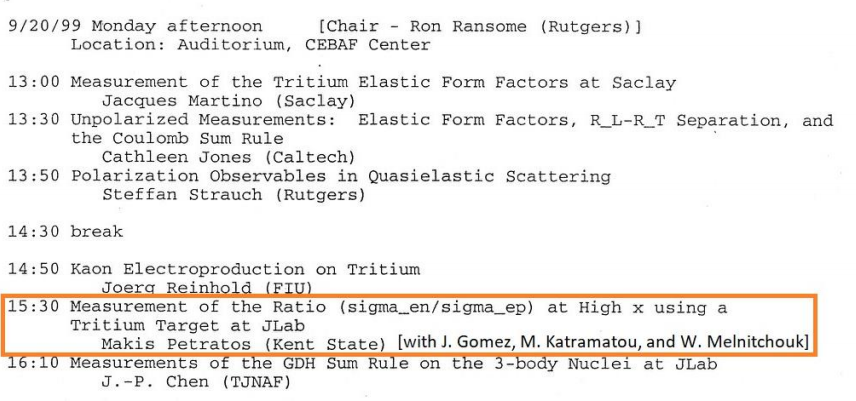
\includegraphics[width =12cm]{../images/pac_agenda.png}
\end{figure}
\end{block}
\end{frame}
%----------------------------------------------
%----------------------------------------------
\begin{frame}
\frametitle{Tritium Experiments}
\vspace{-15pt}
\begin{figure}
	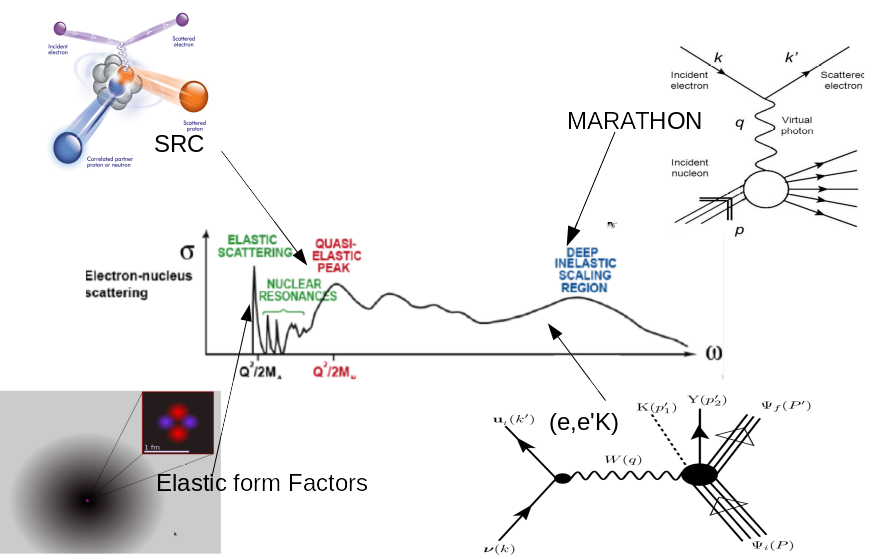
\includegraphics[width =12cm]{../images/tritium_ov}
\end{figure}
\end{frame}
%----------------------------------------------
\begin{frame}
\frametitle{MARATHON}
MeAsurement of $F^n_2/F^p_2, d/u$ RAtios and $A=3$ EMC Effect in Deep Inelastic Electron Scattering off the Tritium and Helium MirrOr Nuclei.
\vspace{-10pt}
\begin{columns}[t]
	
	\column{.45\textwidth} % L column and width
	
	\begin{figure}
		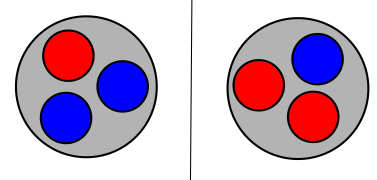
\includegraphics[width =5cm]{../images/mirror}
	\end{figure}
	\vspace{-25pt}
	\begin{figure}
		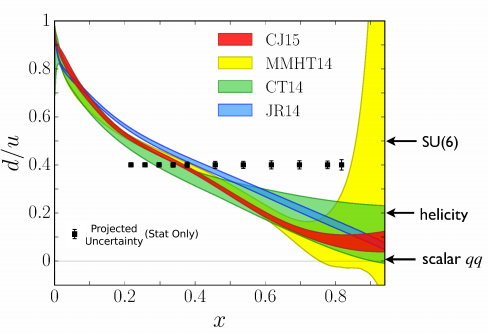
\includegraphics[width=5cm]{../images/d_u}
		\caption{d/u quark distribution ratios}
	\end{figure}
	
	\column{.55\textwidth} % Right column and width
	\begin{itemize}
		\item Lightest and simplest mirror system
		\begin{itemize}
			\item  Number of protons in $^3H =$ neutrons in $^3He$
		\end{itemize}
		\item Differences in the nuclear effects are small
		\item Improve the current measurement and understanding of $F^n_2/F^p_2$ ratio
		\item Restrict the assumptions and parameters made in the model calculations of the down to up quark distribution ratio
	\end{itemize}
	
	
\end{columns}
\end{frame}

%----------------------------------------------------
%----------------------------------------------
\begin{frame}
\frametitle{Deep Inelastic Scattering (DIS)}
\begin{columns}[c] % The "c" option specifies centered vertical alignment while the "t" option is used for top vertical alignment
	
	\column{.45\textwidth} % Left column and width
	\begin{figure}
		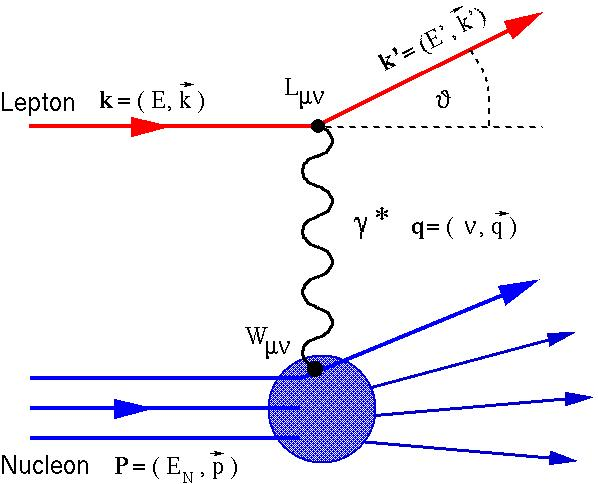
\includegraphics[width =5cm]{../images/DIS}
	\end{figure}
	
	
	\column{.5\textwidth} % Right column and width
	\begin{itemize}
		\item Momentum Transfer $ Q^2 \equiv 4EE' sin \frac{\theta}{2} $
		\item Bjorken X $(X_{bj}/x) = \frac{Q^2}{2\nu M}$
		\item $\sigma_{eN} = \frac{\alpha^2}{eE^2sin^4(\frac{\theta}{2})} [\frac{F_2}{\nu}cos^2\frac{\theta}{2} + \frac{2F_1}{M}sin^2\frac{\theta}{2}] $
		\item Invariant Mass $W^2 = 2M\nu + M^2 - Q^2$
		\item $W^2 > 4 \rightarrow$ DIS
	\end{itemize}
	
	
	
\end{columns}
\end{frame}
%----------------------------------------------
\begin{frame}
\frametitle{$\frac{F_2^n}{F_2^p}$ in the Quark Parton Model}
\vspace{-15pt}

\begin{figure}
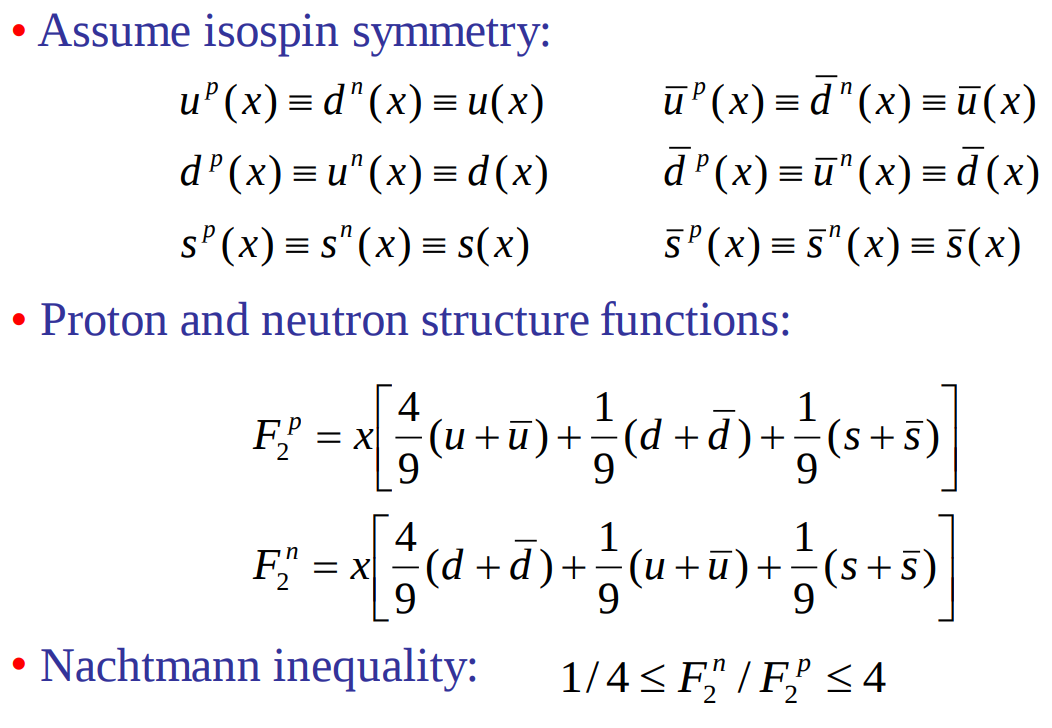
\includegraphics[width =11.5cm]{../images/parton_mod.png}
\end{figure}

\end{frame}
%----------------------------------------------


\begin{frame}

\vspace{-15pt}

	\begin{figure}
		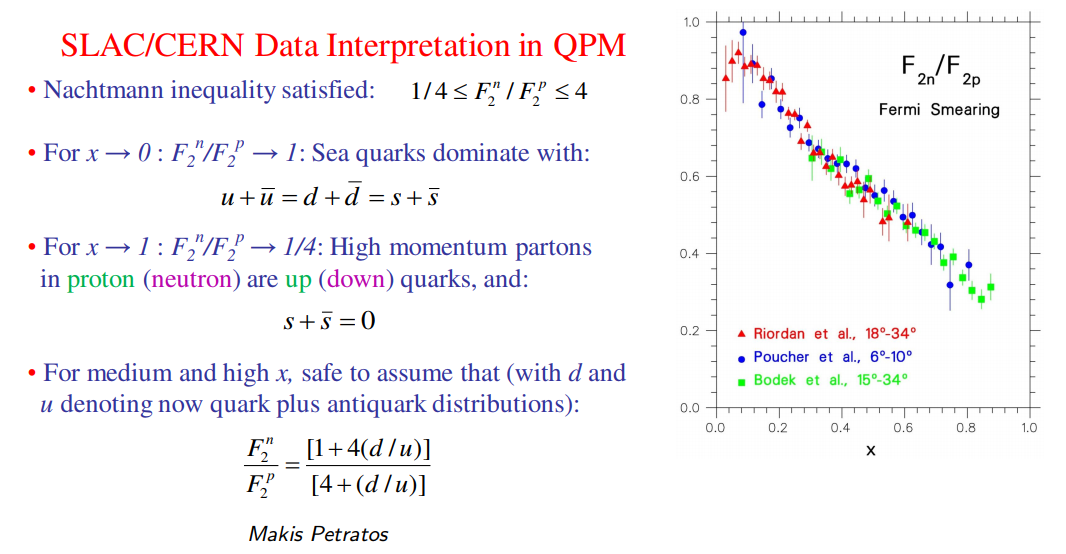
\includegraphics[width =12.5cm]{../images/slac_cern_inter.png}
	\end{figure}

\end{frame}


\begin{frame}
\frametitle{d/u quark ratios}
\vspace{-15pt}

\begin{figure}
	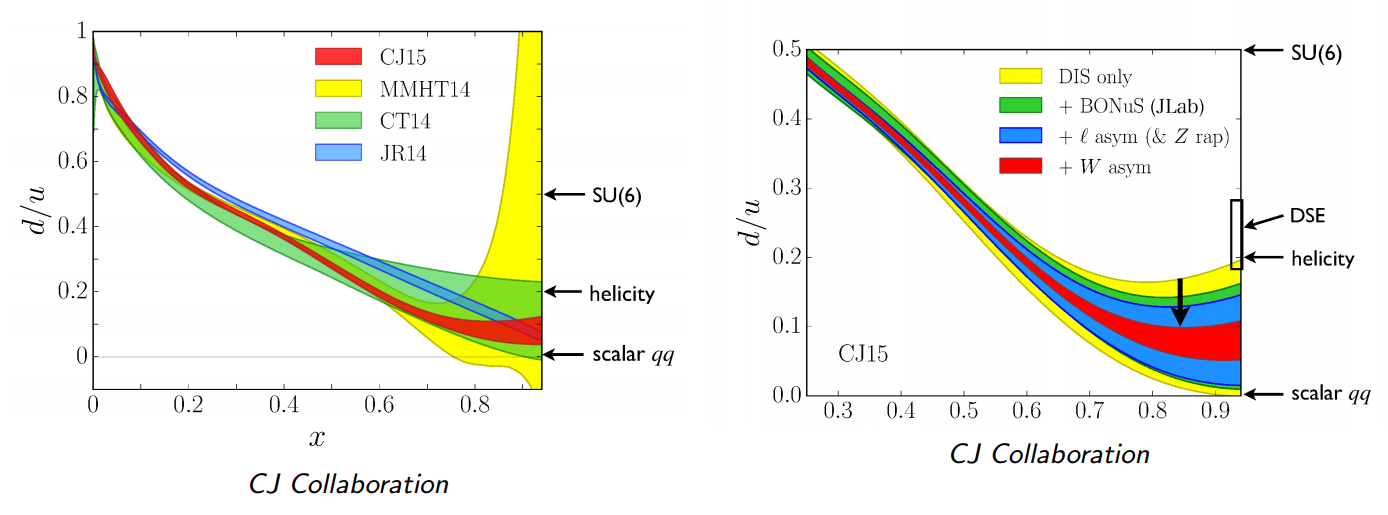
\includegraphics[width =12.5cm]{../images/d_u_plots.png}
\end{figure}

\end{frame}
%----------------------------------------------
%----------------------------------------------
\begin{frame}{EMC Effect}

\begin{figure}
	\caption{\label{EMC_slac} SLAC experiment E139 .}
	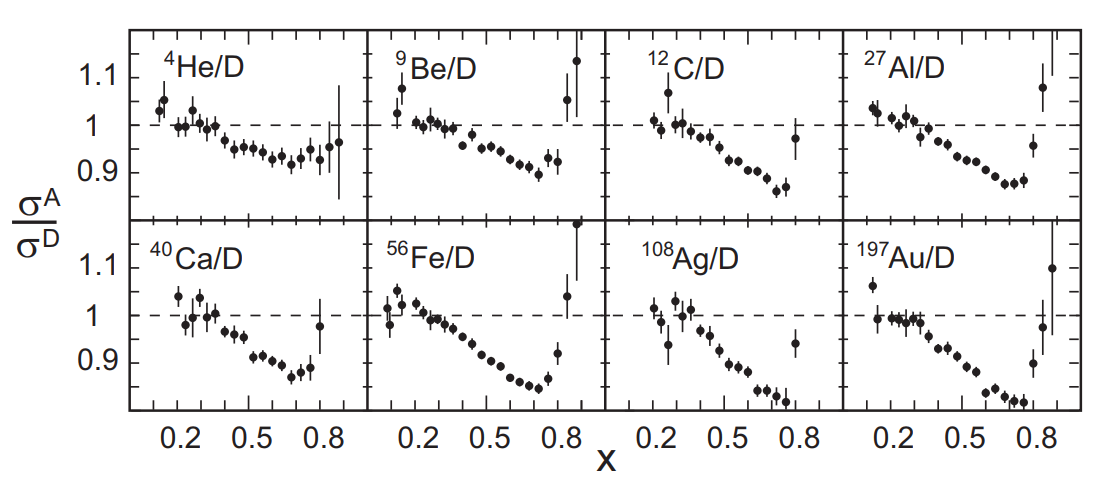
\includegraphics[width =12cm]{../images/EMC_slac_horiz.png}
\end{figure}


\end{frame}

%----------------------------------------------
\begin{frame}{EMC Effect}
\begin{columns}
\column{.5\textwidth} % Left column and width
\vspace{-15pt}
\begin{figure}
	\caption{\label{E03103} JLab experiment "EMC in light Nuclei". J.Seely, A. Daniel et al}
	\vspace{-20pt}
	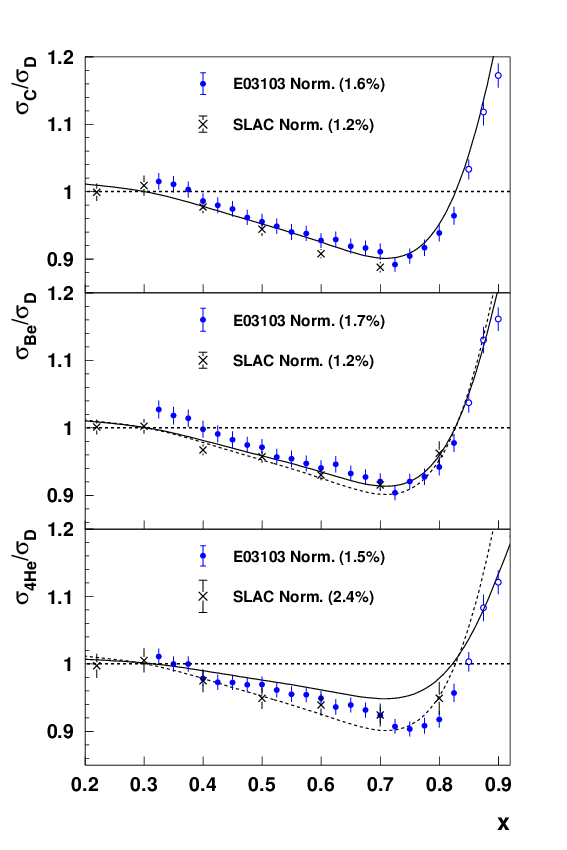
\includegraphics[width =5cm]{../images/carbon_be_he4}
\end{figure}
\column{.55\textwidth} % Left column and width
\hspace{10pt}
\begin{figure}
	\caption{\label{E03103_1} EMC as a function of Nuclear Density. J.Seely, A. Daniel et al}
	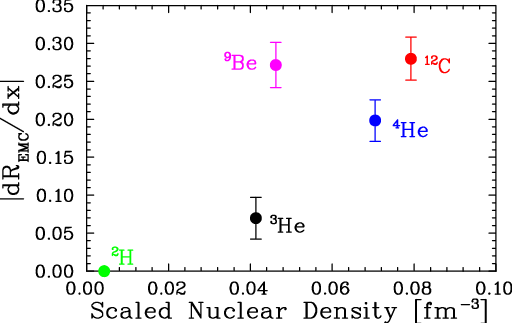
\includegraphics[width =6cm]{../images/PRL_slopes}
\end{figure}
\centering
Scaled by $\frac{\left(A-1\right)}{A}$
\end{columns}
\end{frame}

%----------------------------------------------




%----------------------------------------------
\begin{frame}
\frametitle{The JLab MARATHON Tritium Collaboration}
\vspace{-15pt}

\begin{figure}
	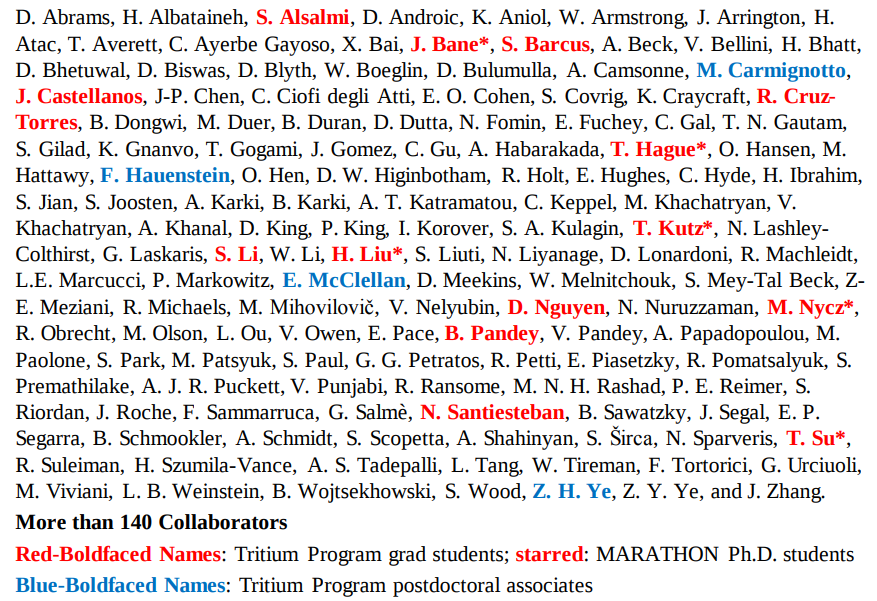
\includegraphics[width =11.5cm]{../images/collabos_ppl.png}
\end{figure}

\end{frame}
%----------------------------------------------
%----------------------------------------------
\begin{frame}
\frametitle{The JLab MARATHON Tritium Collaboration}
\vspace{-15pt}

\begin{figure}
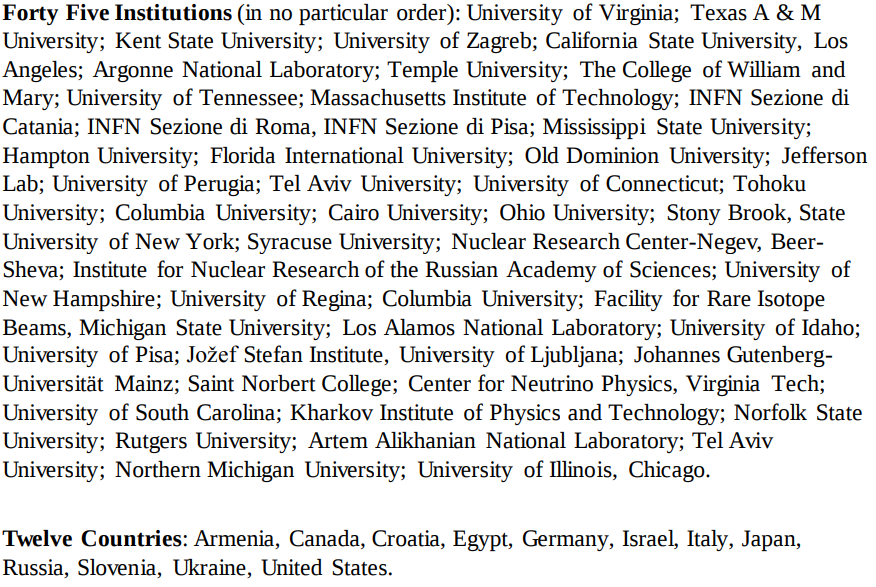
\includegraphics[width =11.5cm]{../images/callabos_un.png}
\end{figure}

\end{frame}
%----------------------------------------------


\begin{frame}
\frametitle{Hall A $\&$ The HRSs}

\begin{block}{}
	Use CEBAF(Continues Electron Beam Facility) to provide 10.6 GeV beam for electron scattering. 
\end{block}
\vspace{-20pt}
\begin{columns}
\column{0.45\textwidth}
\begin{figure}
	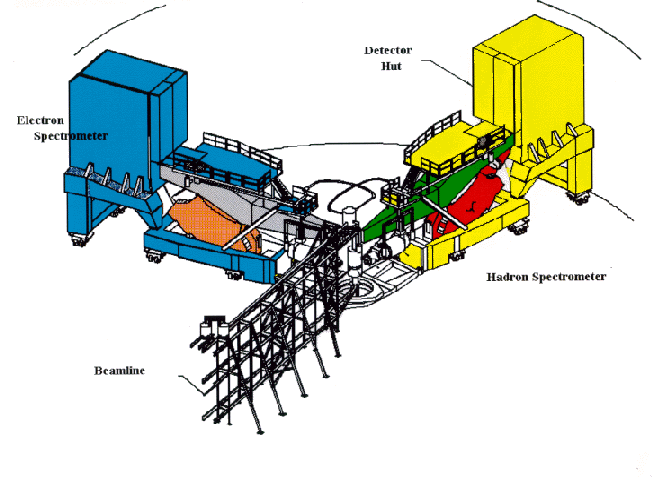
\includegraphics[width=6cm]{../images/Halla_img}
\end{figure}
\column{0.45\textwidth}
\begin{figure}
	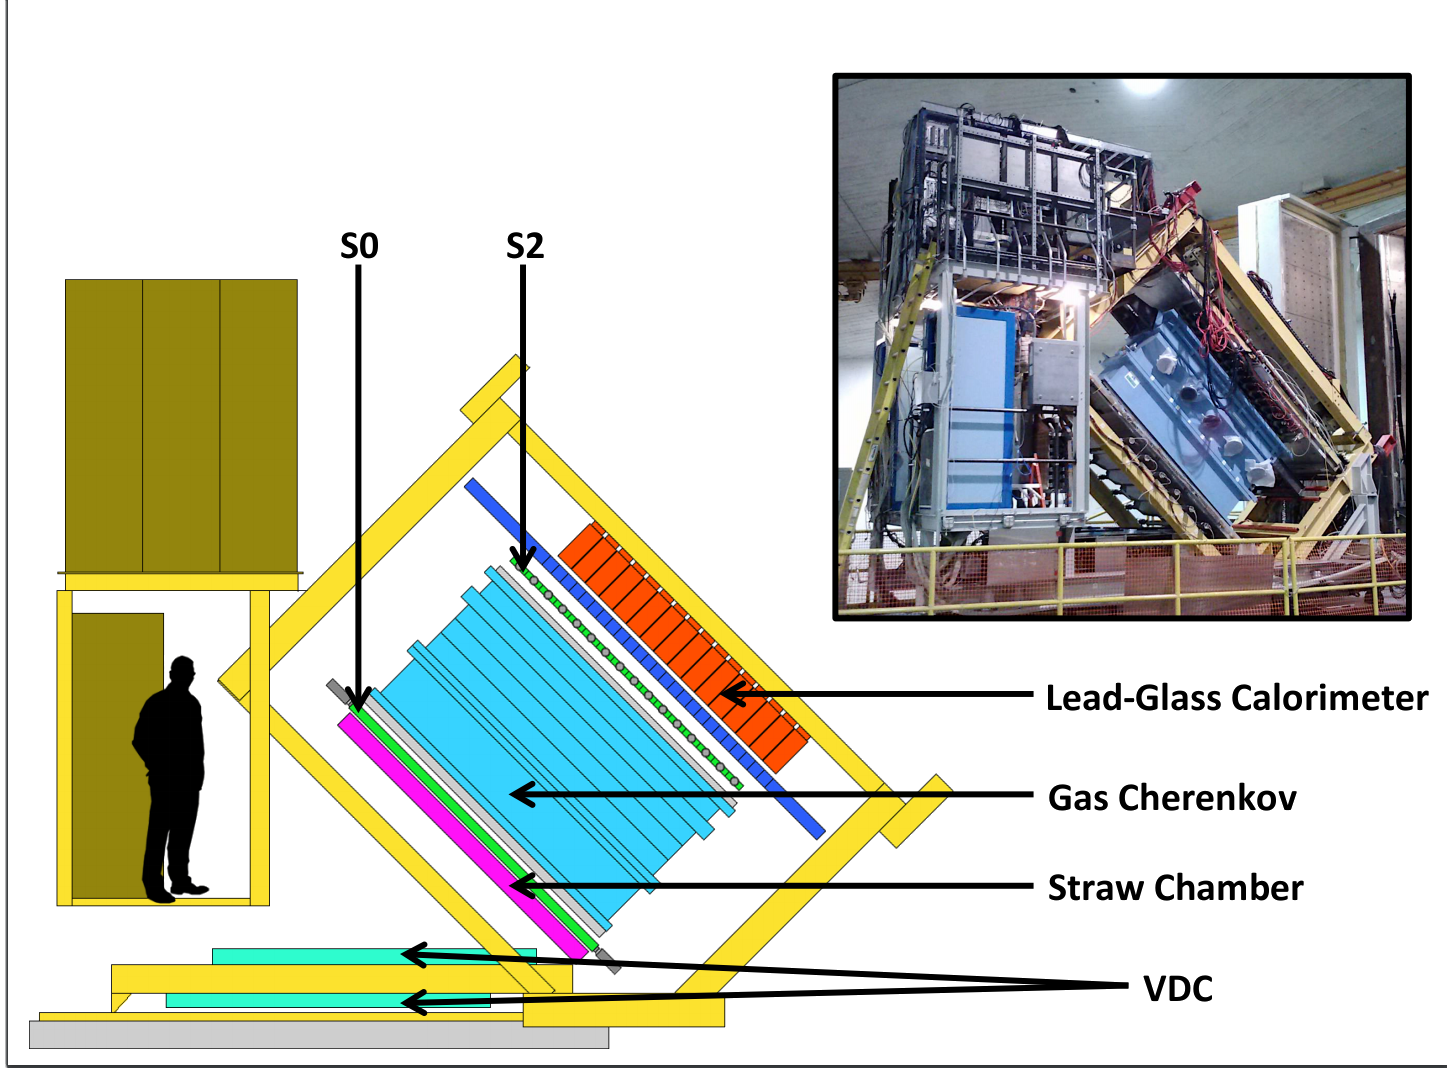
\includegraphics[width=6cm]{../images/HRS_cartoon}
\end{figure}

\end{columns}
\end{frame}
%---------------------------------------------------------------
\begin{frame}
\frametitle{Tritium Target Cell}
\begin{columns}
	\column{0.45\textwidth}
	First tritium target at JLab
	\begin{itemize}
		\item Thin Al entrance and exit windows ~0.01 inches
		\item 1090Ci of Tritium (0.1 g)
		\item 25 cm long
		\item Tritium Cell was filled in Savannah River
		\item 40 kelvin Helium is used to cool an attached heat sink
	\end{itemize}
	\column{0.45\textwidth}
	\begin{figure}
		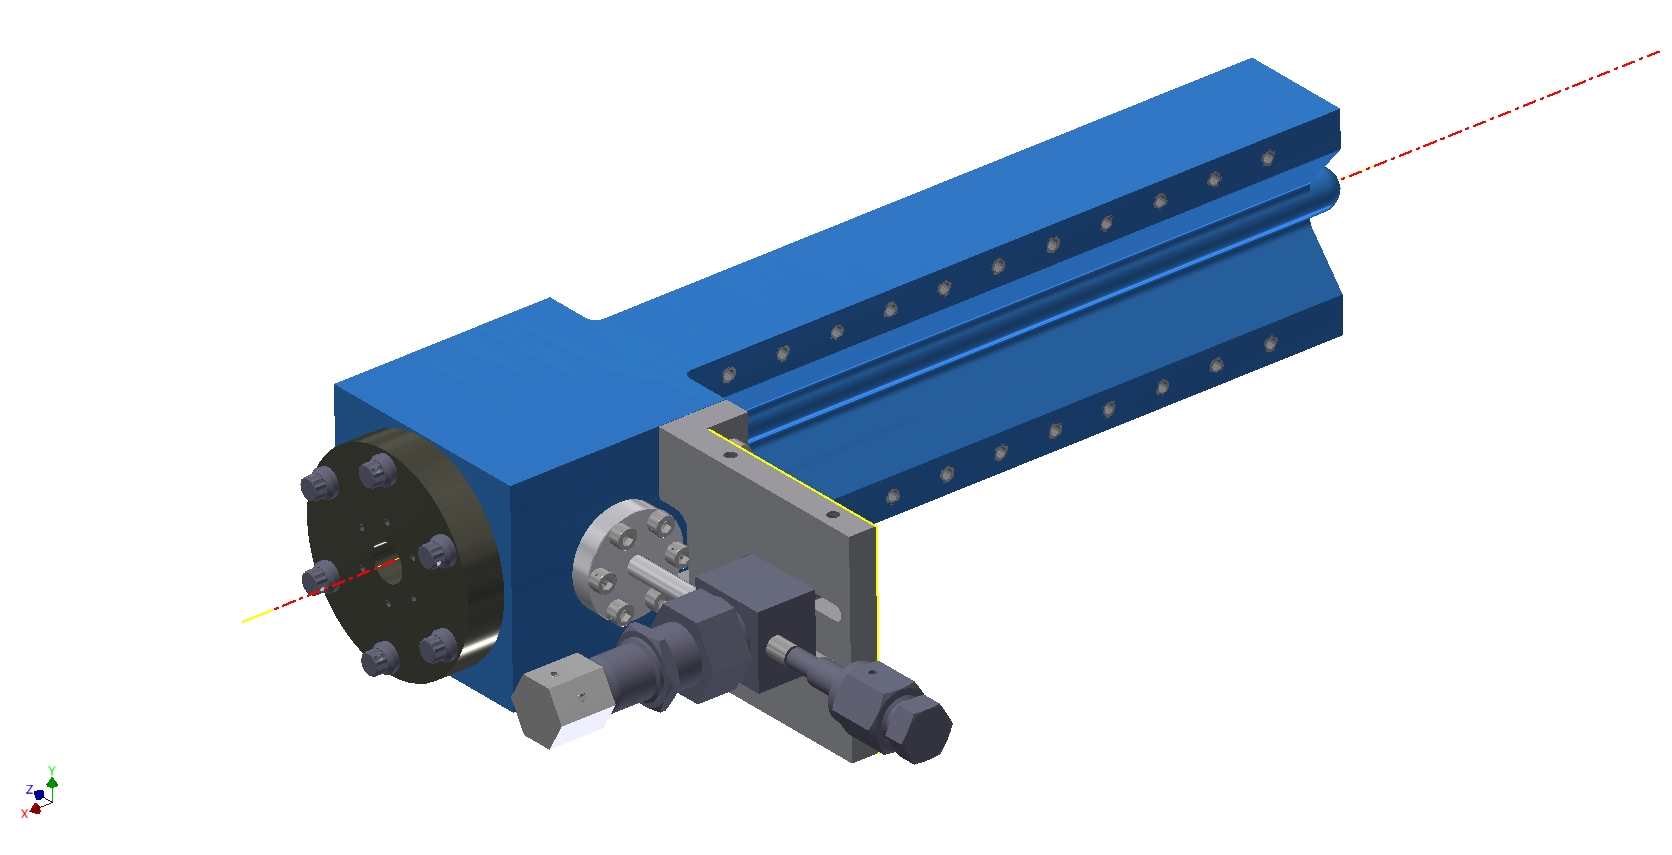
\includegraphics[width=5cm]{../images/tgt_cell}
	\end{figure}
	\vspace{-10pt}
	\begin{figure}
		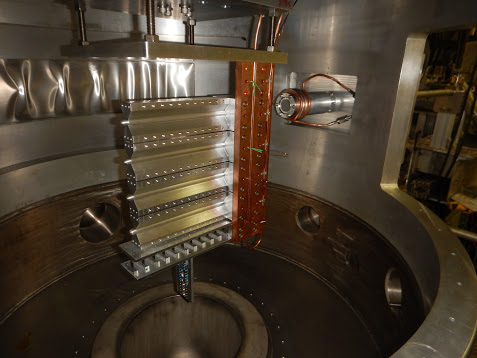
\includegraphics[width=5cm]{../images/tag_lat}
	\end{figure}
\end{columns}
\end{frame}

%-----------------------------------------------


\begin{frame}
\frametitle{The Run Period}
	\vspace{-20pt}
	\begin{columns}
		\column{0.35\textwidth}	
		\begin{figure}
			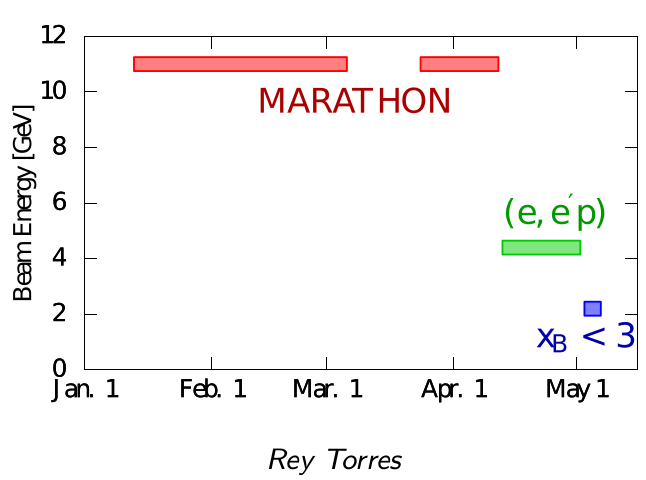
\includegraphics[width=4.5cm]{../images/run_per}
		\end{figure}
		\column{0.65\textwidth}
		\vspace{-10pt}
		\begin{itemize}
			\item Ran from January 11th to April 12th of 2018.
			\item Gaseous Tritium, Deuterium, Helium-3, and Hydrogen
			\item Single Carbon Foil, Carbon foil with hole, and multi-foil
			\item Rotated through targets to achieve equal statics and reduce the impact of unforeseen circumstances
		\end{itemize}
	\end{columns}
	\begin{figure}
	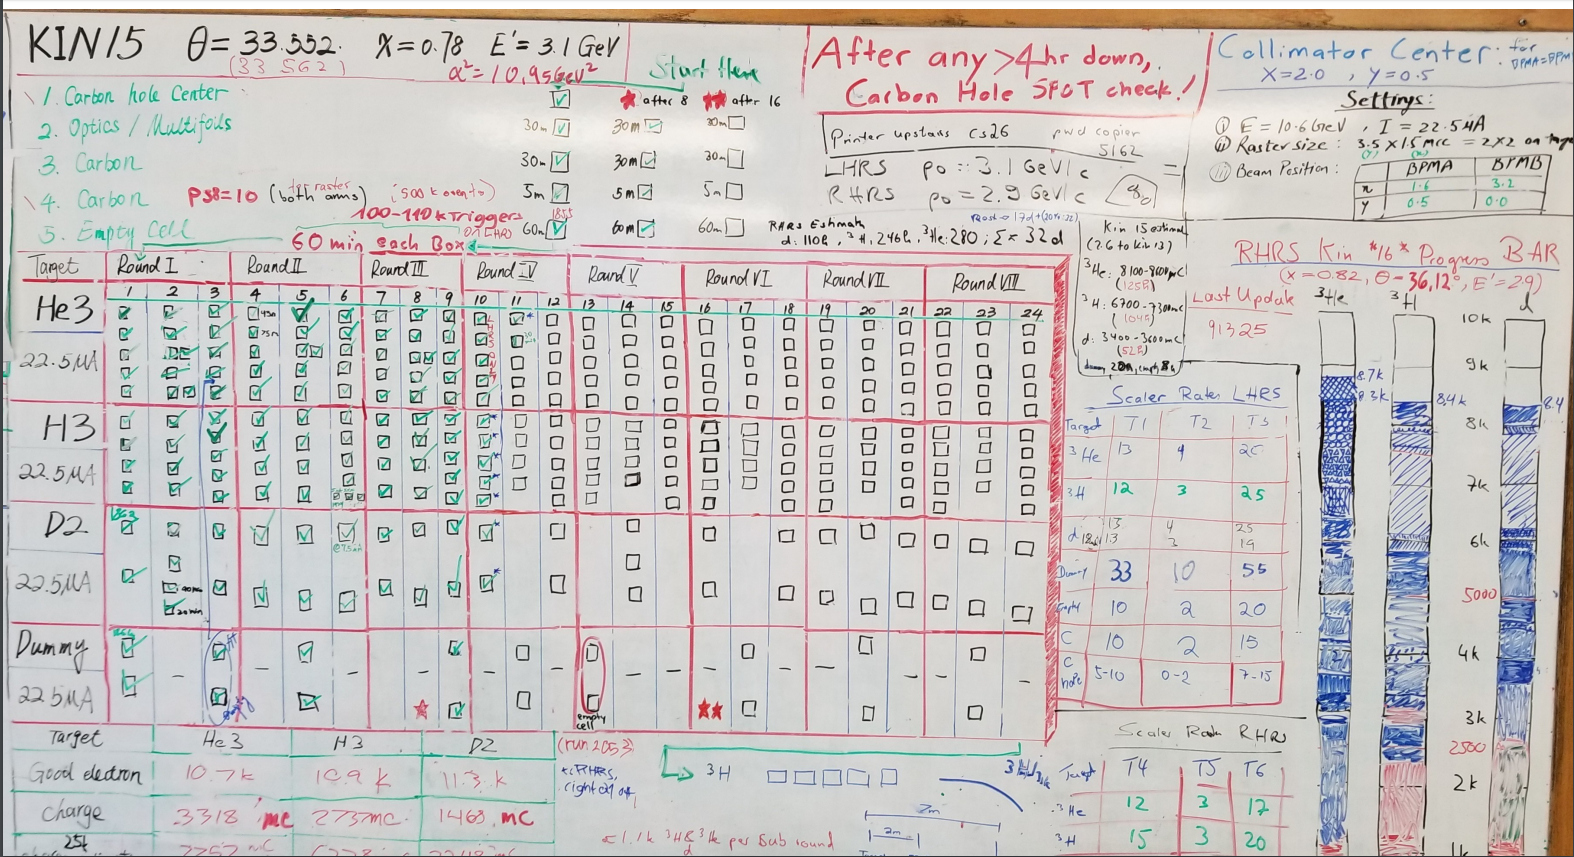
\includegraphics[width=6.5cm]{../images/whiteboard_2_20}
	\end{figure}
\end{frame}

%--------------------------------------------------------
\begin{frame}
\frametitle{Major Miscues}
\begin{block}{}
	\begin{itemize}
		\item Right Arm Dipole failed on January 11th
		\begin{itemize}
			\item Return the dipole to functionally the following day
			\item 01/13 - Dipole failed again, causing a chain reaction with the Left arm
			\item Solution could not be found quickly
			\item Change of Kinematic plan to use single HRS.
			\item Recovered RHRS on 01/16 - Set to take data at theta of 36.12$^\circ$,  $x$ of 0.82 
		\end{itemize}
		\item A Transformer Failed on March 5th 
		\begin{itemize}
			\item Recovered on March 23rd
			\item Spring run Period extended by 18 days
			\item MARATHON took opportunistic data during recovery period 
		\end{itemize}
	\end{itemize}
\end{block}

\end{frame}
%------------------------------------------------------------------

\begin{frame}
\begin{columns}[t]
	\column{0.55\linewidth}
%	\vspace{-10pt}
	
	\begin{figure}
		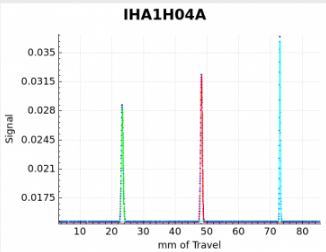
\includegraphics[width=4.5cm]{../images/harpscan1}
	\end{figure}
	
	\vspace{-10pt}
	\begin{figure}
		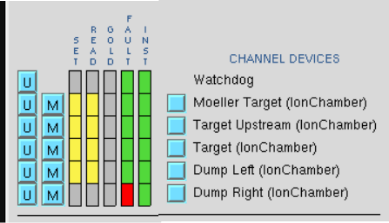
\includegraphics[width=4.5cm]{../images/ION}
	\end{figure}
	\column{0.5\linewidth}
	\vspace{-20pt}
	\begin{block}{Tritium Safety Requirements}
		\begin{itemize}
			\item Harp and BPM Check!
			\item Ion Chamber functionality test
			\item Beam Center
			\item Raster Size calibration. 
		\end{itemize}	
	\end{block}	
	\vspace{-10pt}
	\begin{figure}
		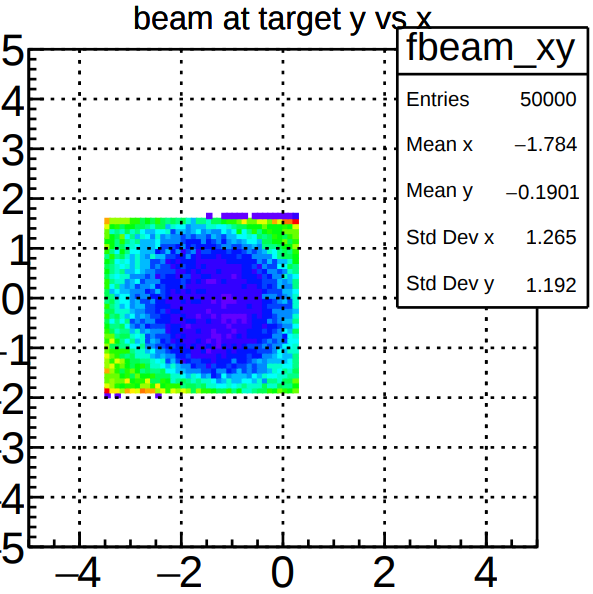
\includegraphics[width=5cm]{../images/spot}
	\end{figure}	
\end{columns}
\end{frame}
%------------------------------------------------------------------
\begin{frame}
\frametitle{Systematics: $^3H $ Decay}
	\begin{block}{$^3H \rightarrow ^3He$}
		\begin{columns}
			\column{0.45\textwidth}
			\begin{equation*}
			 	\tau^3He = 4500 \pm 8 days
			 \end{equation*}		 	
			 \\
			 \begin{equation*}
			 	c = \frac{\eta_{^3He}} {\eta_{tot}}
			 \end{equation*}
			 \\
 			 \begin{equation*}
				 \sigma_{^3H} = \big(\frac{\sigma_{tot}}{\sigma_{^3He}}\big) \big(\frac{1}{1-c}\big) -  \big(\frac{1}{1-c}\big)  
			 \end{equation*}
			 \column{0.55\textwidth}
		 	\begin{figure}
			 	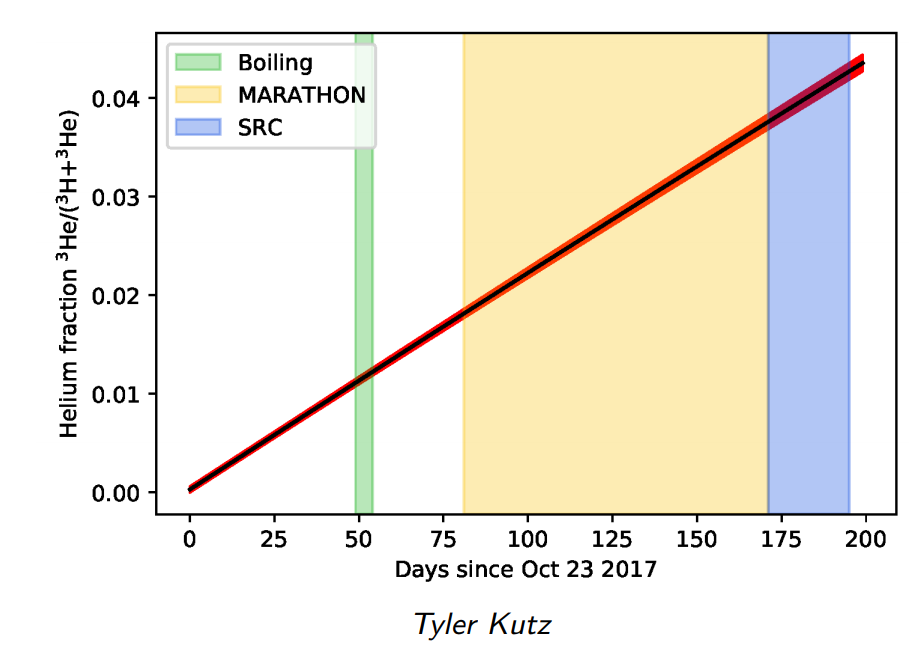
\includegraphics[width=6cm]{../images/beta_decay.png}
			 \end{figure}
		\end{columns}
	\end{block}
\end{frame}



%------------------------------------------------------------------
\begin{frame}
\frametitle{Systematics: Endcaps}
	\vspace{-10pt}
\begin{block}{}
	\begin{figure}
		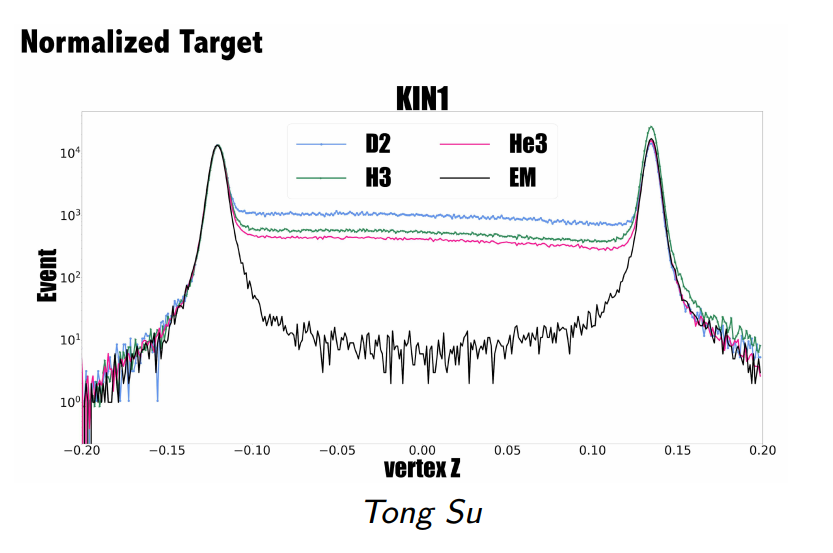
\includegraphics[width=8cm]{../images/em_tgt_comp.png}
	\end{figure}

\begin{itemize}
	\item Extract ratio of the normalized yield from the gas cell to that of the empty cell
\end{itemize}

\end{block}
\end{frame}
%------------------------------------------------------------------

\begin{frame}{Systematics: Density Fluctuations}
	\vspace{-15pt}
	\begin{block}{}
	\begin{figure}
		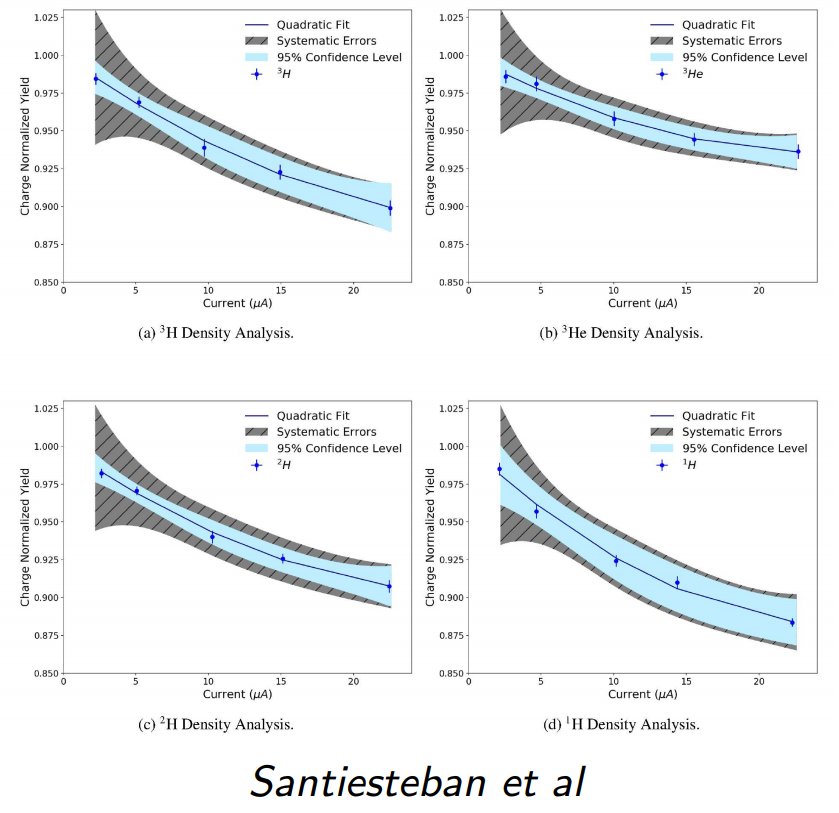
\includegraphics[width=8cm]{../images/density_cor.png}
	\end{figure}
	\end{block}
\end{frame}
%------------------------------------------------------------------

\begin{frame}{Charge Symmetric back ground}
\vspace{-20pt}
\begin{block}{}
	\begin{columns}
		\column{0.45\textwidth}
		\begin{itemize}
			\item High energy photons decay into an e$^+$e$^-$ pairs
			\item Account for the pair produced e$^-$ by detecting the pair produced e$^+$
			\item HRS positive polarity - kinematics 1,2 and 3
			\item Fit results with an exponential function to determine the contamination factor at high $x_{Bj}$ kinematics.

		\end{itemize}
		\column{0.45\textwidth}
		\begin{figure}
			
		\end{figure}
		\vspace{-40pt}
		\begin{figure}
			\textbf{Pair Production}
			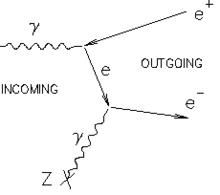
\includegraphics[width=3.0cm]{../images/pp_FD.png}
		\end{figure}
		\vspace{-20pt}
		\begin{figure}
			\textbf{Tritium positron contamination}
			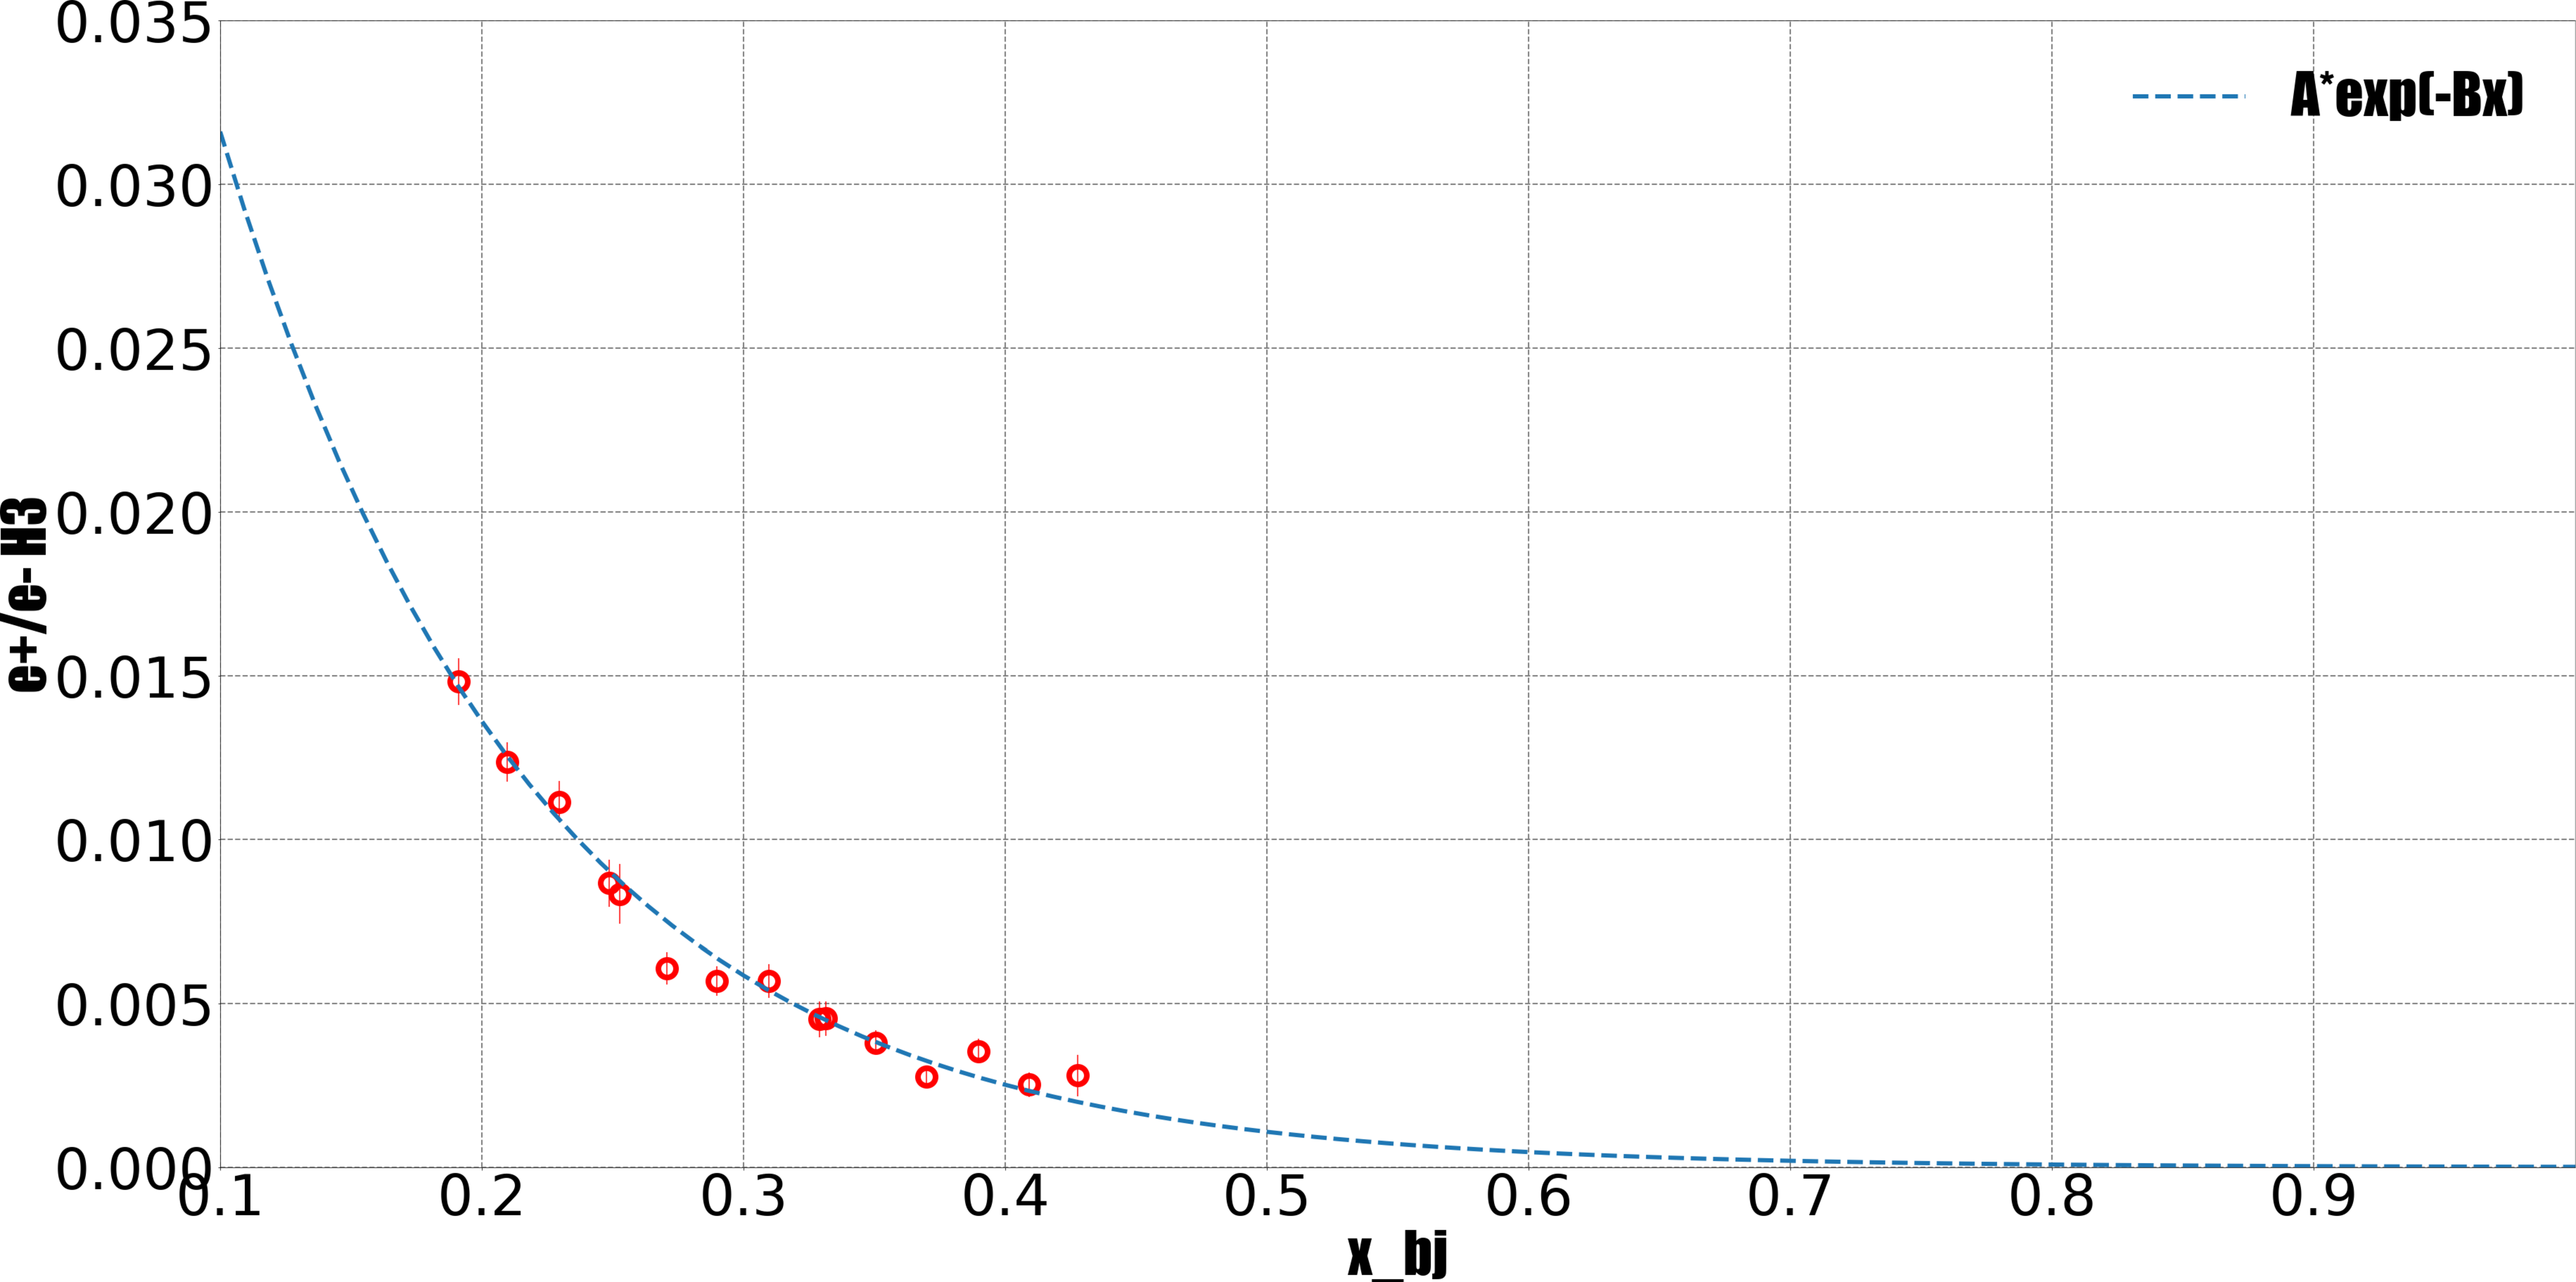
\includegraphics[width=5.0cm]{../images/positron_H3_bane.pdf}
		\end{figure}
		
	\end{columns}
	
\end{block}
\end{frame}
%------------------------------------------------------------------


\begin{frame}{}
\frametitle{d/p and $^3H/^3He$}
\vspace{-10pt}
\begin{columns}
	\column{0.5\textwidth}
	\begin{figure}
		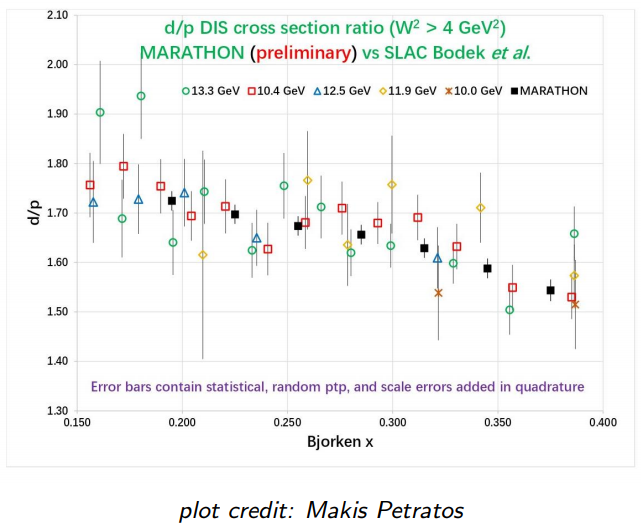
\includegraphics[width=6cm]{../images/d_p_makis.png}
	\end{figure}
	\column{0.5\textwidth}
	\begin{figure}
		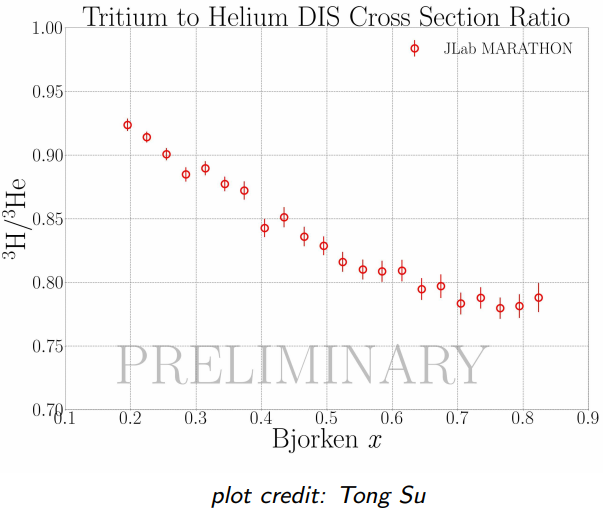
\includegraphics[width=6cm]{../images/H_H.png}
	\end{figure}
\end{columns}
\end{frame}

\begin{frame}{Extracting F2}

\begin{figure}
	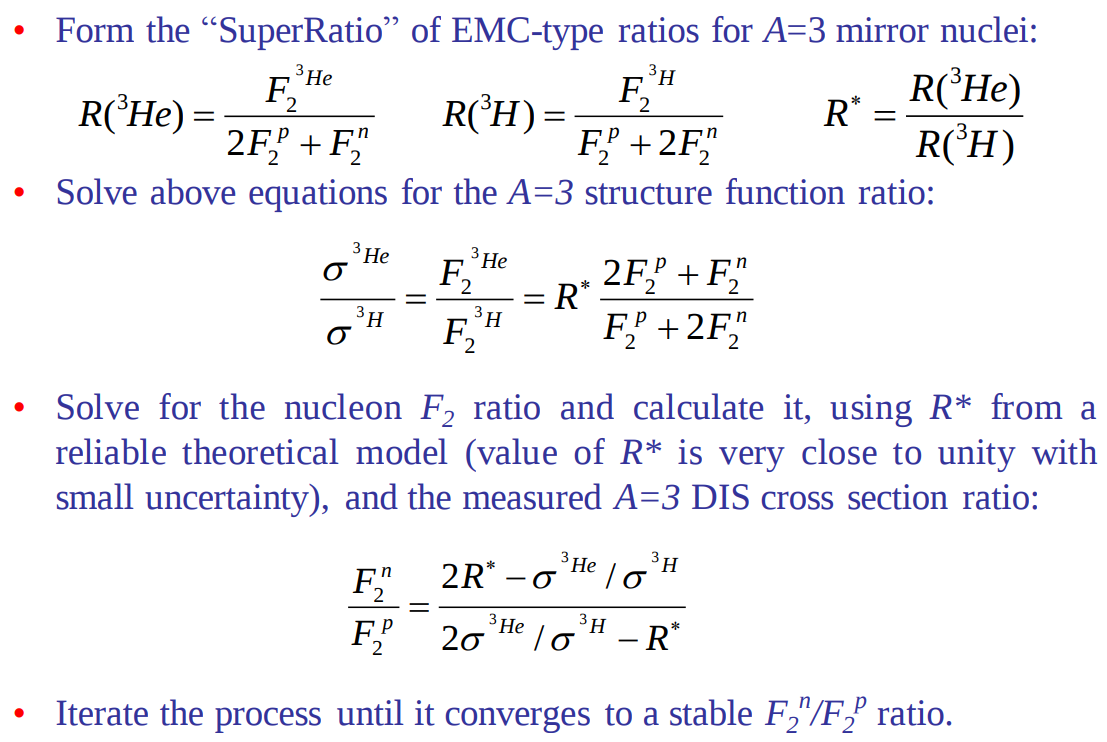
\includegraphics[width=10cm]{../images/f2ext.png}
\end{figure}
\end{frame}

\begin{frame}{Extracting F2}
\vspace{-10pt}
\begin{figure}
	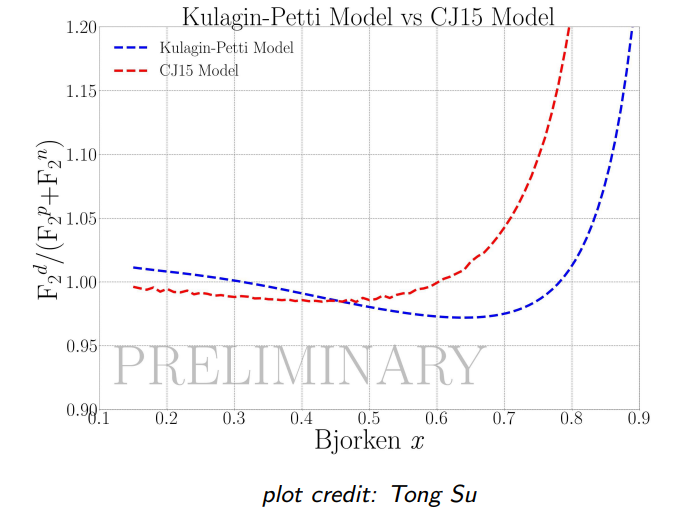
\includegraphics[width=10cm]{../images/kp_cj.png}
\end{figure}
\end{frame}


\begin{frame}{$\frac{F_2^n}{F_2^p}$ for D/p}
\vspace{-20pt}
\begin{figure}
	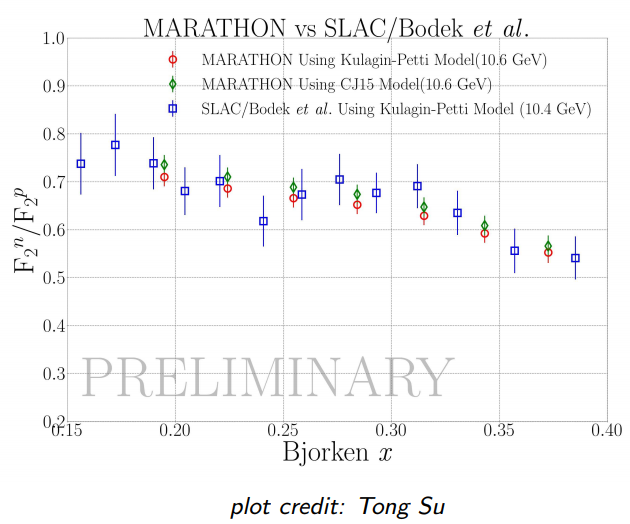
\includegraphics[width=9.5cm]{../images/ff_al.png}
\end{figure}
\end{frame}

\begin{frame}{$\frac{F_2^n}{F_2^p}$}
\vspace{-20pt}
\begin{figure}
	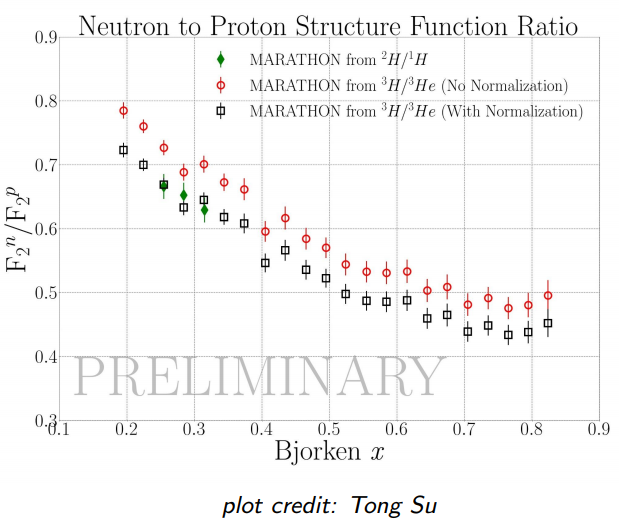
\includegraphics[width=9.5cm]{../images/fff.png}
\end{figure}
\end{frame}

\begin{frame}{}
\begin{columns}
	\column{0.5\textwidth}
	\begin{block}{Monte Carlo}
		\begin{itemize}
			\item Generate events in target space
			\item Pass through detector aperture
			\item Use optics matrix to project back to target from focal plane.
			\item Tune Simulation to match detector response
			\item Adjust initial parameters
			\item Use model to weight events
			\begin{itemize}
				\item Deep Inelastic and resonance region from Bodek Fit 
				\item Quasi elastic model of F1F2QE09 
			\end{itemize}    
		\end{itemize}
	\end{block}
	\column{0.45\textwidth}
	\vspace{-20pt}
	\begin{figure}
		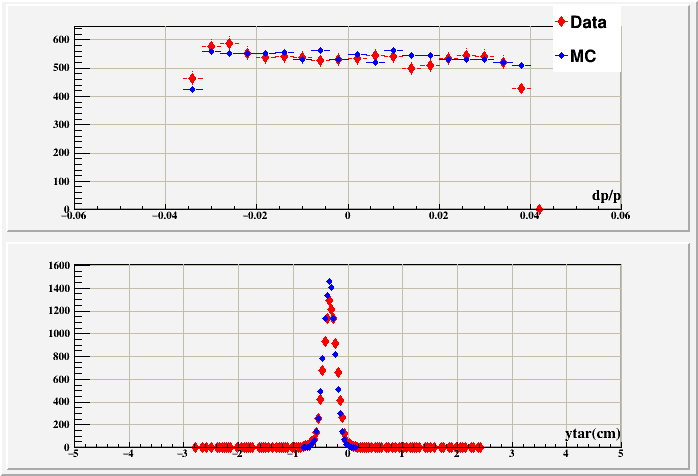
\includegraphics[width=6cm]{../images/dp_ytar_1207.png}
	\end{figure}
	\vspace{-30pt}
	\begin{figure}
		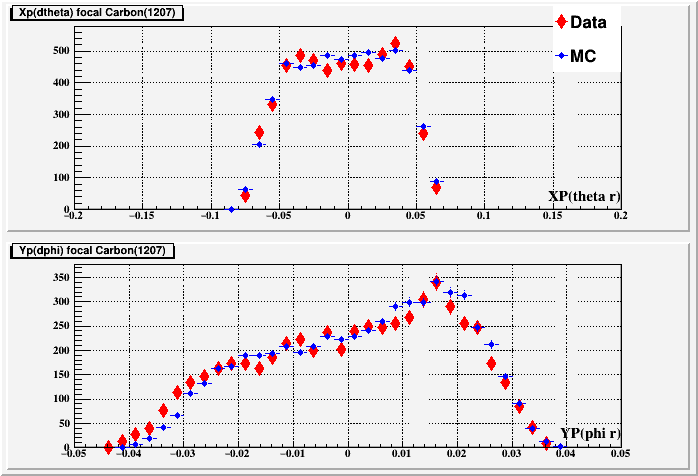
\includegraphics[width=6cm]{../images/xp_yp_foc_1207.png}
	\end{figure}
\end{columns}
\end{frame}
%------------------------------------------------------------------


\begin{frame}{EMC Effect}
\vspace{-20pt}
\begin{figure}
	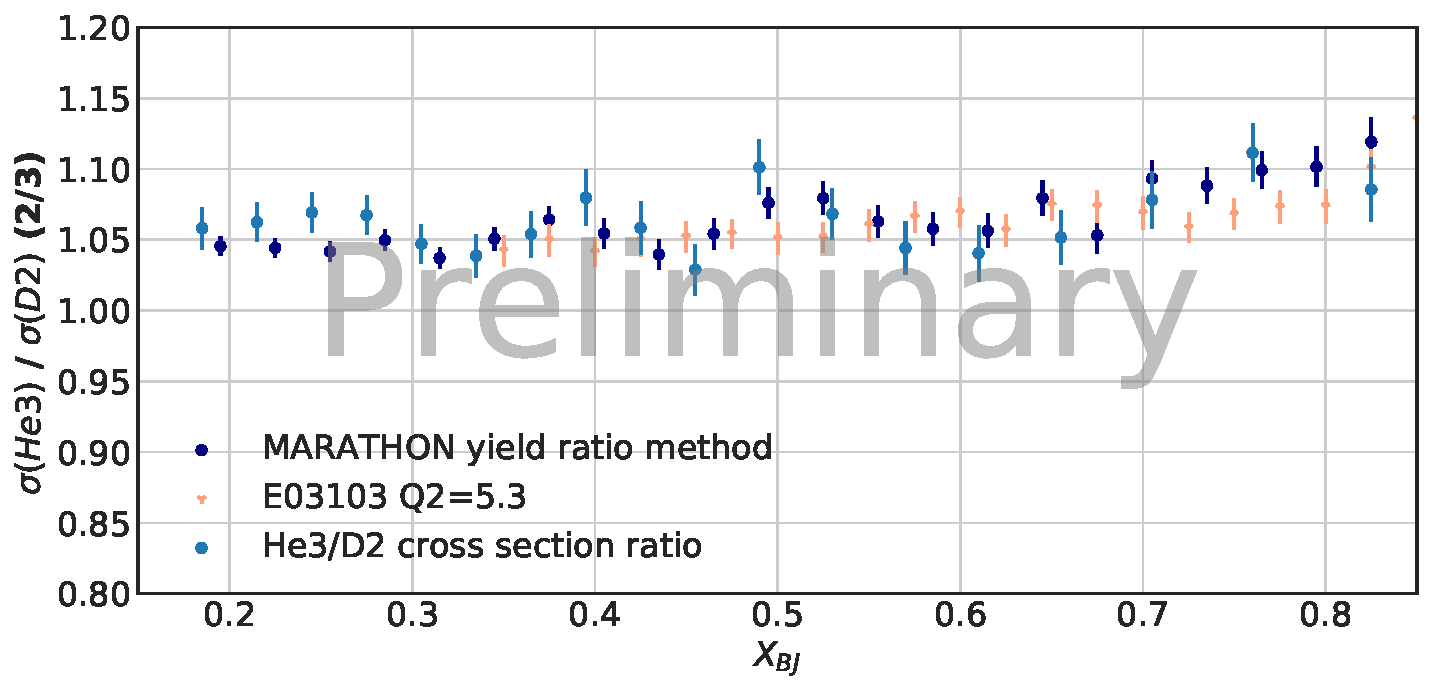
\includegraphics[width=8.5cm]{../images/He3_EMC.pdf}
\end{figure}
\vspace{-20pt}
\begin{figure}
	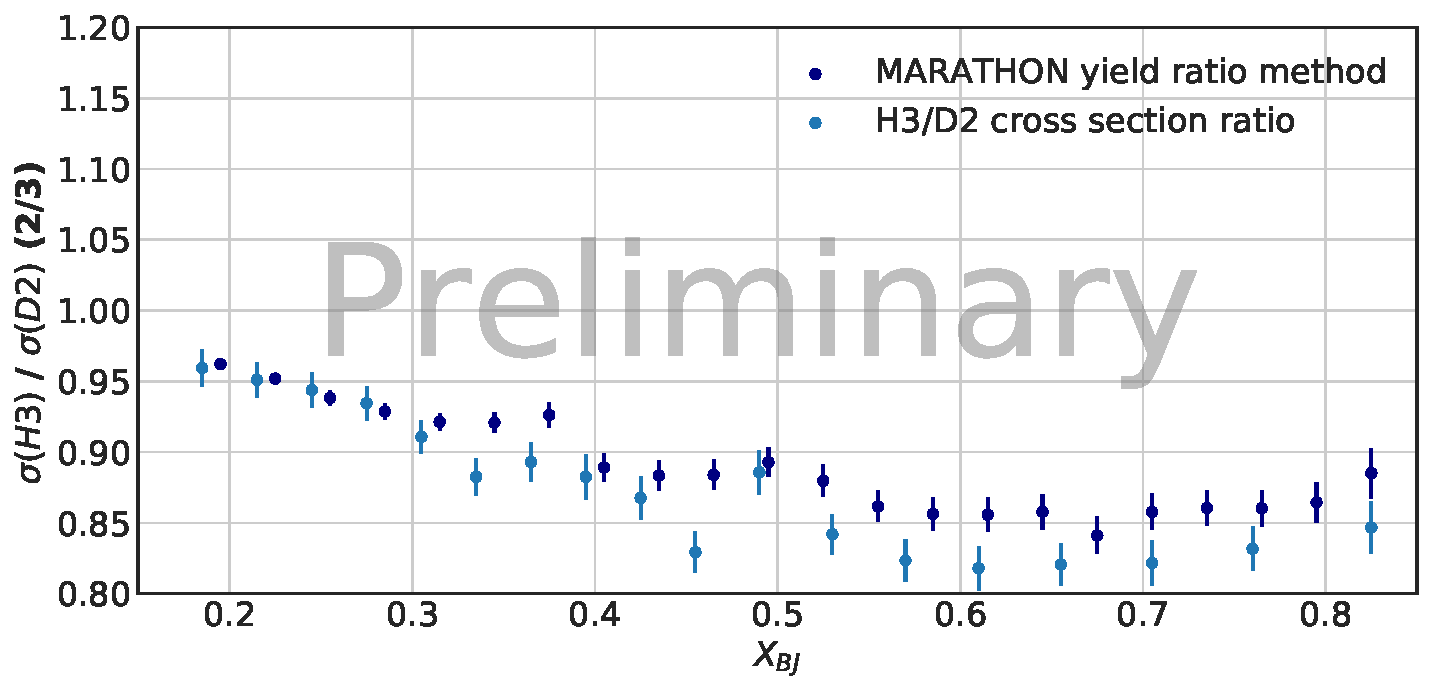
\includegraphics[width=8.5cm]{../images/H3_EMC.pdf}
\end{figure}
\end{frame}


%------------------------------------------------------------------

\begin{frame}
\begin{block}{Thank you!!}
	\begin{itemize}
		\item MARATHON students
		\item Tritium collaboration
		\item Hall A Collaboration
		\item Hall C Collaborators that took shifts during MARATHON
		\item Nadia Fomin and Doug Higinbotham
	\end{itemize}
\end{block}
\end{frame}


\end{document} 

%----------------------------------------------
\begin{frame}
\frametitle{$F^n_2/F^p_2 $}
\vspace{-15pt}
\begin{block}{Slack/CERN Data}
	\begin{figure}
		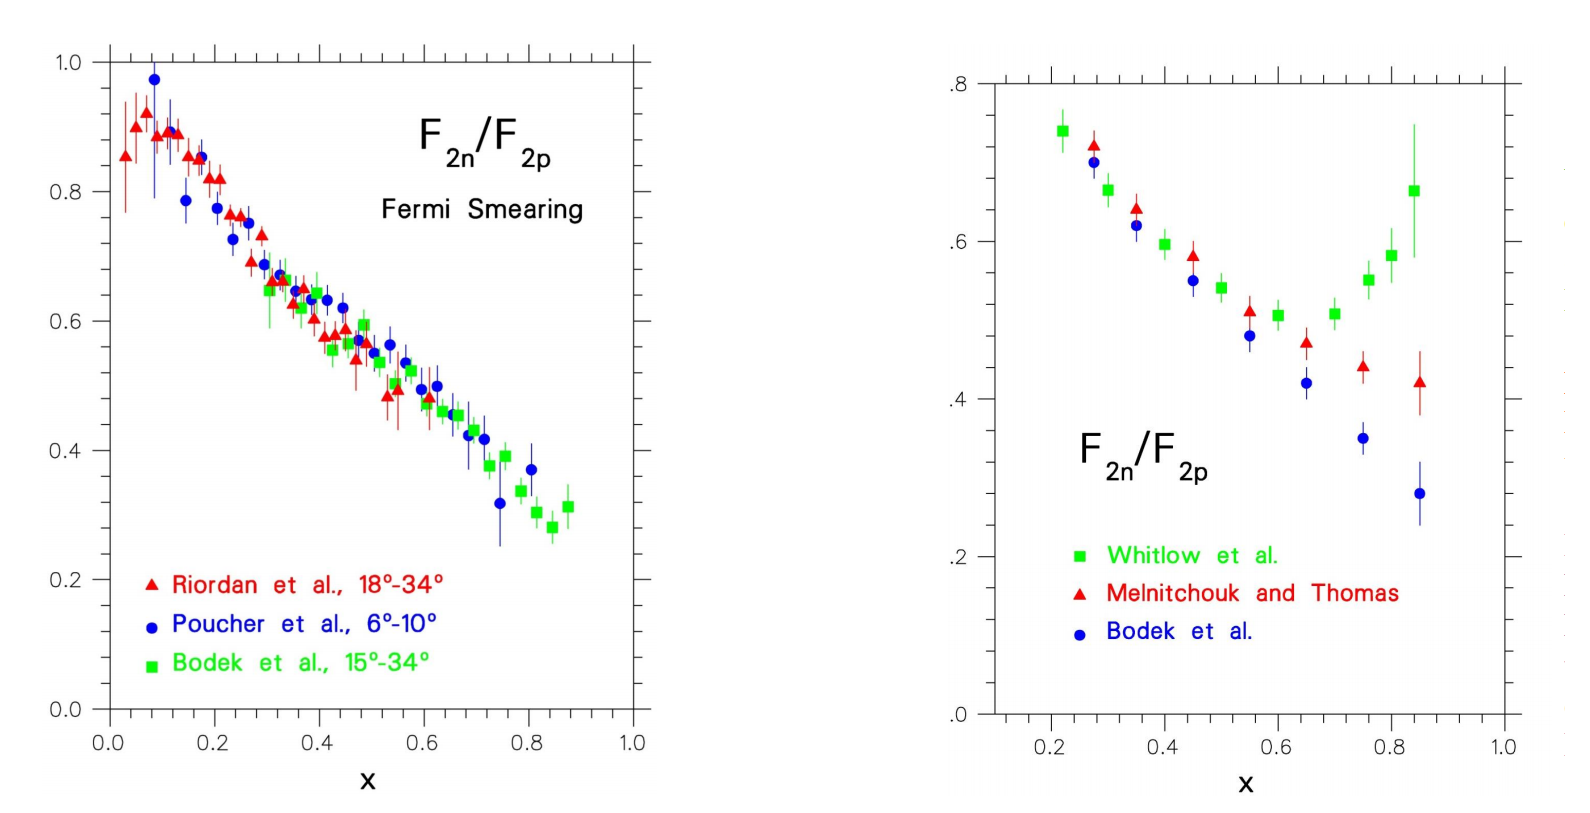
\includegraphics[width =11.5cm]{../images/f2n_fnp_plots.png}
	\end{figure}
\end{block}
\end{frame}
%----------------------------------------------
\begin{frame}{Systematic Studies}
\vspace{-20pt}
\begin{columns}
	\column{0.45\textwidth}	
	\begin{figure}\caption{Density Fluctuations}\vspace{-10pt} 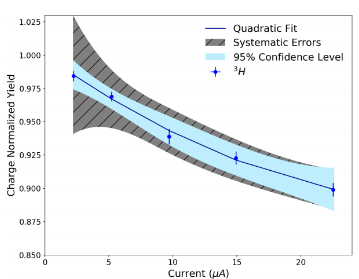
\includegraphics[width=5cm]{../images/dens}\end{figure}
	\vspace{-10pt}
	\begin{figure}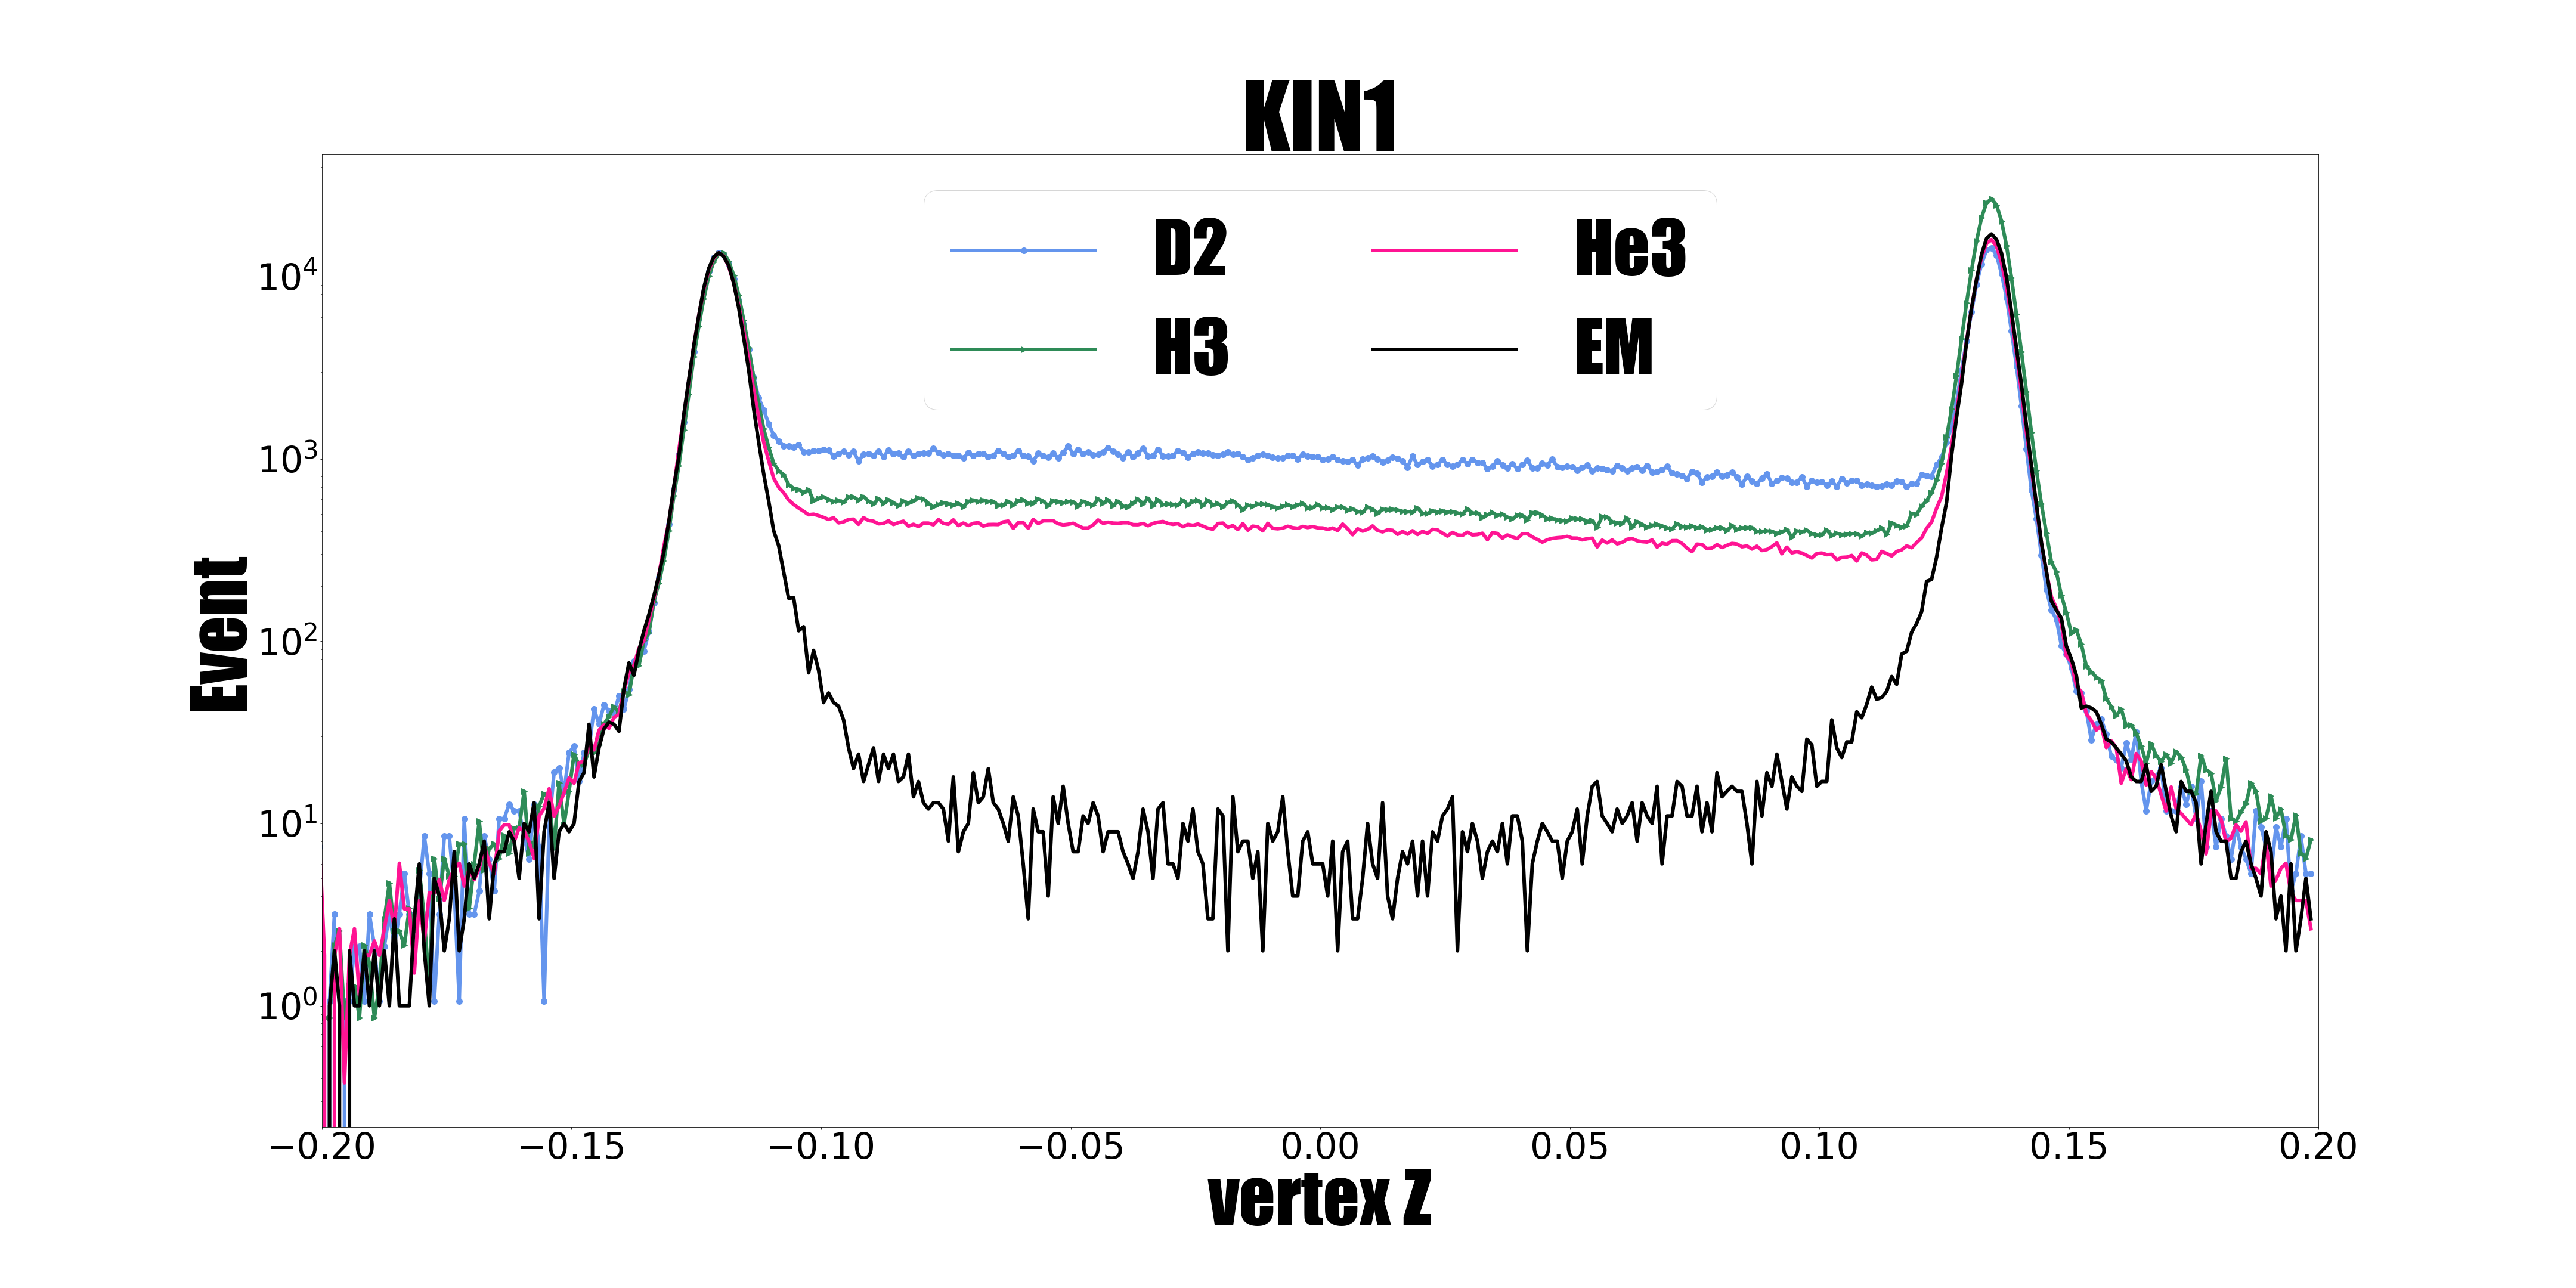
\includegraphics[width=5cm]{../images/ecc}
		\caption{End Cap Contamination}\end{figure}
	\column{0.55\textwidth}	
	\begin{figure}\caption{Tritium beta decay} 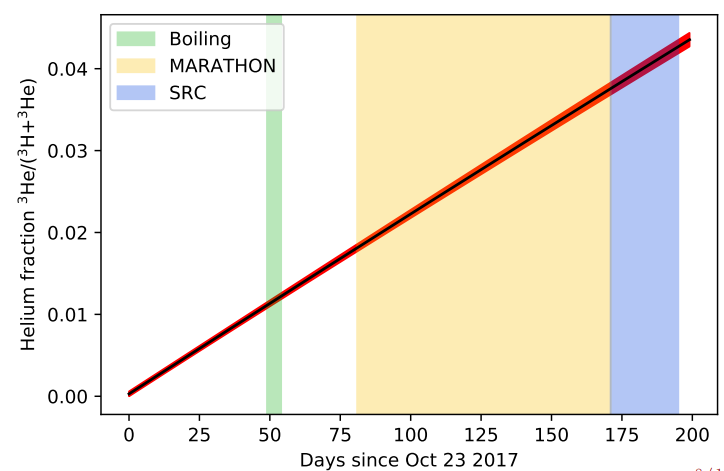
\includegraphics[width=5cm]{../images/decay}\end{figure}
	\vspace{-10pt}
	\begin{figure}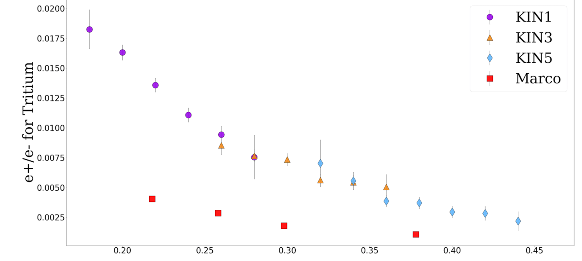
\includegraphics[width=5cm]{../images/pos}
		\caption{Charge Symmetric background}\end{figure}
\end{columns}
\end{frame}


\begin{frame}{}
\begin{columns}
	\column{0.5\textwidth}
	\begin{block}{Monte Carlo}
		\begin{itemize}
			\item Generate events in target space
			\item Pass through detector aperture
			\item Use optics matrix to project back to target from focal plane.
			\item Tune Simulation to match detector response
			\item Adjust initial parameters
			\item Use model to weight events
			\begin{itemize}
				\item Deep Inelastic and resonance region from Bodek Fit 
				\item Quasi elastic model of F1F2QE09 
			\end{itemize}    
		\end{itemize}
	\end{block}
	\column{0.45\textwidth}
	\vspace{-20pt}
	\begin{figure}
		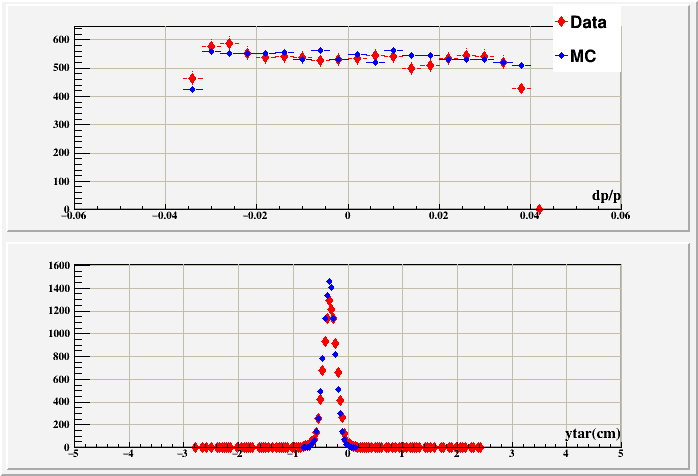
\includegraphics[width=6cm]{../images/dp_ytar_1207.png}
	\end{figure}
	\vspace{-30pt}
	\begin{figure}
		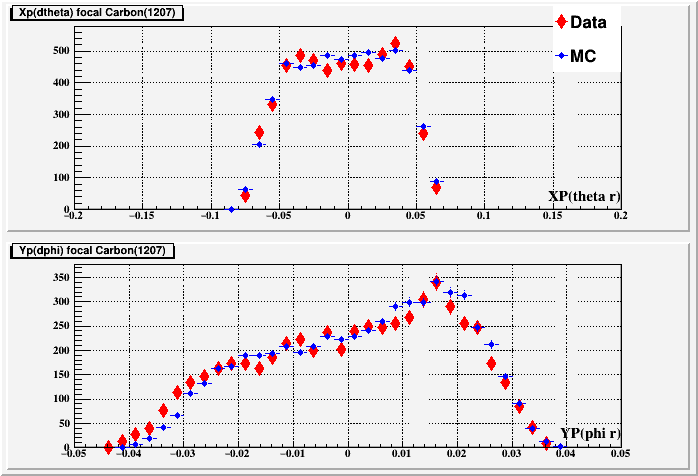
\includegraphics[width=6cm]{../images/xp_yp_foc_1207.png}
	\end{figure}
\end{columns}
\end{frame}
%------------------------------------------------------------------
\begin{frame}
\vspace{-10pt}
\begin{block}{Acceptance Studies}
\begin{figure}
	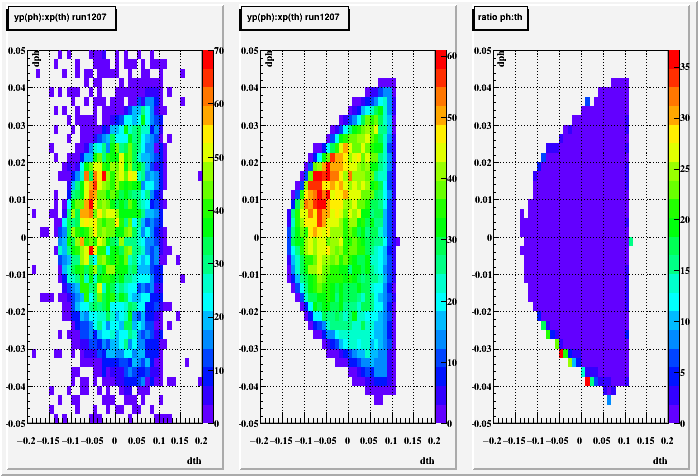
\includegraphics[width=10cm]{../images/xpyp_comp}
\end{figure}
\vspace{-20pt}
\begin{itemize}
	\item Determine where the acceptance is understood the best
	\item Use comparison plots to make efficient fiducial cuts. 
\end{itemize}

\end{block}
\end{frame}



\begin{frame}
\frametitle{References}
\footnotesize{
	\begin{thebibliography}{99} % Beamer does not support BibTeX so references must be inserted manually as below
		\bibitem[Higinbotham D., 2013]{cc} Douglas Higinbotham (2013) 
		\newblock The EMC effect still puzzles after 30 years
		\newblock \emph{Cern Courier} April 2013.
		
		\bibitem[J. Gomez et al., 1994]{slac_emc} J. Gomez et al. (SLAC-E139)  
		\newblock \emph{Phys. Rev D}  49 (1994) 4348 
		
		\bibitem[J.Seely, A. Daniel et al]{E3103} J.Seely, A. Daniel et al (2013) 
		\newblock New Measurements of the EMC Effect in Very Light Nuclei
		\newblock \emph{nucl-ex/0904.4448}.
		
		\bibitem[J. Alcorn et al.]{nim} J. Alcorn et al, (2004)
		\newblock Basic instrumentation for Hall A at Jefferson Lab
		\newblock NIM A 522(2004) 294-346
		\bibitem[A. Bodek and U.K. Yang]{bodek} A. Bodek and U.K. Yang
		\newblock \emph{Nuclear Physics B, Procc. Suppl. 112 (2002) 70-76 }
		
		\bibitem[P. Bosted and E. Christy]{F1F} Bosted $\&$ Christy (2008)
		\newblock Phys. Rev. C 77, 065206 (2008)
		
	\end{thebibliography}
}
\end{frame}
%------------------------------------------------

